% \documentclass[aps,pre,showpacs,superscriptaddress]{revtex4}
\documentclass[12pt,aip,cha,reprint,nofootinbib]{revtex4-1}
\usepackage{amsfonts,amssymb,amsmath,times}%
\usepackage{graphicx}
\usepackage{bm}
\usepackage{enumerate}
\usepackage{color}

% \linespread{1}

\begin{document}

% \title{Estimation of coupling directions by means of ordinal partition transition network approaches}
\title{Ordinal partition transition network based complexity measures for inferring coupling direction and delay from time series}

\author{Yijing Ruan}
	\affiliation{Department of Physics, East China Normal University, Shanghai, 200062, China}

\author{Reik V. Donner}
	\affiliation{Department of Water, Environment, Construction and Safety, Magdeburg--Stendal University of Applied Sciences, Breitscheidstra{\ss}e 2, 39114 Magdeburg, Germany}
	\affiliation{Potsdam Institute for Climate Impact Research (PIK) -- Member of the Leibniz Society, Telegrafenberg A31, 14473 Potsdam, Germany}

\author{Shuguang Guan}
    \affiliation{Department of Physics, East China Normal University, Shanghai, 200062, China}

\author{Yong Zou}
\email[corresponding author: ]{yzou@phy.ecnu.edu.cn}
    \affiliation{Department of Physics, East China Normal University, Shanghai, 200062, China}

\date{\today}

\begin{abstract}
It has been demonstrated that the construction of ordinal {\color{red}partition} transition networks (OPTNs) from time series provides a prospective approach to improve our understanding of the underlying dynamical system. In this work, we introduce several OPTN based complexity measures to infer the coupling direction between two dynamical systems from pairs of time series. For several examples of coupled stochastic processes, we demonstrate that our approach is able to successfully identify interaction delays of both unidirectional and bidirectional coupling configurations. Moreover, we show that the causal interaction between two coupled chaotic H\'enon maps can be captured by the OPTN based complexity measures for a broad range of coupling strengths before the onset of synchronization. Finally, we apply our method to two real-world observational climate time series, disclosing the interaction delays underlying the temperature records from two distinct stations in Oxford and Vienna. Our results suggest that ordinal {\color{red}partition} transition networks can be used as complementary tools for causal inference tasks and provide insights into the potentials and theoretical foundations of time series networks. 
\end{abstract}

\pacs{05.45.Ac, 05.45.Tp, 89.75.Fb}
\maketitle

\begin{quotation} 
The construction of transition networks from time series is one of the most widely spread methods for time series analysis based on complex network approaches. Transition networks allow to characterize the intrinsic heterogeneity of the state transition behavior of the system, which provides many novel insights supplementing traditional time series analysis methods. However, most existing works on this topic have focused on disclosing properties of a single time series, which calls for a generalization to multi-variate analysis. Here, we choose the problem of identifying coupling direction as a showcase to demonstrate that measures quantifying the heterogeneity of state transitions in ordinal {\color{red}partition} transition networks can successfully capture unidirectional and bidirectional coupling between paradigmatic models of dynamical systems as well as real-world time series. 
\end{quotation}

\section{Introduction}
Over the last decade, various complex network approaches have been proposed in the literature to understand the complexity of nonlinear time series \cite{Bradley2015c,Kantz97,ZouPR2018}. The first step of constructing complex networks from time series is to identify proper definitions for network nodes and links \cite{ZouPR2018}. Given the great variety of possible definitions, this leads to diverse transformation approaches including recurrence networks \cite{Marwan2009,Donner2010NJP}, visibility graphs \cite{Lacasa2008}, transition networks \cite{Nicolis2005,McCullough2015} and cycle networks \cite{Zhang2006} as some of the most notable examples. The resulting network representations have been successfully applied to diverse real-world observational time series from various fields, for instance, climate and Earth sciences \cite{Donges2011PNAS,Elsner2009,schleussner2015indications}, fluid mechanics and turbulence \cite{Liu2009,Gorski2015,Gao2015a,Gao2016b,Manshour2015a}, medicine \cite{Ramirez2013,Subramaniyam2015}, financial markets \cite{Flanagan2016}, or astrophysics \cite{Zou2014a,Zou2014}. A comprehensive summary of recent developments can be found in ref.~\cite{ZouPR2018}.

In this work, we focus on the application of transition networks from time series. This class of time series network representations comprises several different ways for defining the nodes of a transition network upon a given data set. In general, the nodes of a transition network correspond to certain discrete states or patterns, and directed links are established if one of these nodes is followed by the other with non-zero (empirical) probability along the observed trajectory of the system under study. One common way to define a network node is to utilize  symbolic encoding, which transforms a time series into a set of $K$ discrete states or patterns (``symbols") $\{\pi_1, \dots , \pi_K \}$. The resulting transition network is a weighted and directed graph, which corresponds to a Markov chain with given transition probabilities between discrete states \cite{Schnakenberg1976}.

Ordinal partition transition networks (OPTN) constitute a specific type of transition networks, where a node is represented by the vector of rank orders of the components of a sequence of observations (referred to as an ordinal pattern), while a weighted link captures the transition frequency between two successive ordinal patterns \cite{McCullough2015,KulpChaos2016,KulpChaos2016b,McCulloughChaos2016,SakellariouChaos2016}. In this regard, OPTNs utilize the framework of ordinal time series analysis, which provides important methodological concepts (such as the permutation entropy of a time series \cite{Bandt2002} or complexity measures based on a similar rationale) and allows building upon the well-developed theory of symbolic methods in the context of dynamical systems theory and nonlinear time series analysis \cite{Daw2003,Finn2003,Amigo2010}. While the classical permutation entropy provides just a single measure taking an integrated view on the heterogeneous succession of ordinal patterns, the OPTN \cite{McCullough2015,KulpChaos2016,McCullough2017b} provides information complementary to the standard ordinal or symbolic analysis of time series by further exploiting the corresponding transition frequencies and their mutual interdependencies more explicitly in various ways provided by complex network theory. Notably, in many dynamical systems, certain ordinal patterns do not appear (forbidden patterns), which is indicative of a deterministic nature of the underlying process \cite{KulpChaos2016b,McCulloughChaos2016,SakellariouChaos2016}. Complexity measures based on OPTNs have accordingly demonstrated to be powerful tools for analyzing real-world time series like such originating from an externally driven diode resonator circuit \cite{McCullough2015} and electrocardiograms (ECGs) \cite{McCullough2017b}.

Recently, the idea of OPTNs has been further extended to study multivariate time series \cite{zhangSciRep2017}. One particular achievement is the construction of cross and joint ordinal partition transition networks for two coupled systems \cite{Guo2018}, which has been demonstrated to successfully characterize different types of synchronization transitions. Along with the observation of such transitions, characterizing directed (and potentially causal) interactions among coupled systems is of great importance to identify the underlying coupling configuration from time series, since coupling direction and strength play important roles in the process of synchronization. From a methodological perspective, the identification of coupling directions and associated delays \cite{Coufal2017} from time series has, however, remained a challenging task so far. As a classical representative of a vast class of methods, the Granger test for causality has become increasingly popular to infer and quantitatively characterize the causal relation among two possibly interacting processes \cite{Granger1969}. Hence, this concept has found a broad range of applications to time series in economy, neuroscience and physics \cite{Ding_Book_2007,Dhamala_prl2008}. In this work, we introduce a different method to identify coupling directions (and, thus, potentially infer causality) in terms of complexity measures of bipartite OPTNs. 

The outline of this paper is as follows: In section \ref{sec:intro}, we provide an introduction on the construction of OPTNs from time series, focusing on two possibly interacting processes. In section \ref{sec:measures}, we propose three new measures to quantify heterogeneity in the linkage patterns of the resulting bipartite OPTNs. Some numerical results for different model systems are presented in section \ref{sec:res}, while the results for two observational temperature recordings at spatially distinct sites are discussed in section \ref{sec:exp} as a real-world example. Finally, our main conclusions are summarized in section \ref{sec:con}. 

\section{Ordinal partition transition networks} \label{sec:intro}
The basic idea underlying the transformation of a time series into an OPTN is illustrated in Fig.~\ref{fig:OPexample}. Given a univariate time series $\{x_t\}_{t=1}^N$ with $\Delta t = t_{i+1} - t_{i}$, we start by following the traditional algorithm to reconstruct its phase space by time delay embedding $\vec{x}_{t} = [x_{t}, x_{t+\tau_d}, \cdots, x_{t+(D-1)\tau_d}]$ with dimension $D$ \cite{Takens1981,Kantz97}. Based on the respective amplitudes of the recorded variable $X$, the resulting rank order among the components of each state vector $\vec{x}_t$ is used to obtain a corresponding symbolic encoding. Here, the order of the resulting ordinal patterns associated with the embedding vectors $\vec{x}_{t}$ is determined by the embedding dimension $D$, i.e., there exist at most $D!$ different patterns, which are denoted by $\pi_1, \pi_2, \dots, \pi_{D!}$. The choice of the embedding parameters $\tau_d$ and $D$ is often based on some standard criteria like the first root of the auto-correlation function of the time series and the false nearest neighbor method, respectively \cite{Kantz97}. In the example shown in Fig.~\ref{fig:OPexample}, we have used $\tau_d = 9$ and $D = 6$, and the embedded state vector $\vec{x}_{9}$ is represented by its associated ordinal pattern $\pi_{80}$ (Fig.~\ref{fig:OPexample}(a)). As we follow the system's trajectory in the accordingly reconstructed state space, we obtain a new state vector that is represented by a new ordinal pattern (here, $\pi_{68}$). The resulting series of ordinal patterns is shown in Fig.~\ref{fig:OPexample}(b). By taking the transitions between the different pairs of possible ordinal patterns from the entire time series, we construct an ordinal transition network of $D!$ vertices and directed edges that are weighted by the corresponding empirical transition frequencies. For convenience, we remove self-transitions (loops) in the network (see the sequence in the bottom panel of Fig.~\ref{fig:OPexample}(b)), which would indicate an enduring dynamics of the underlying process that commonly does not often appear in the case of discrete stochastic processes. 

\begin{figure*}
	\centering
	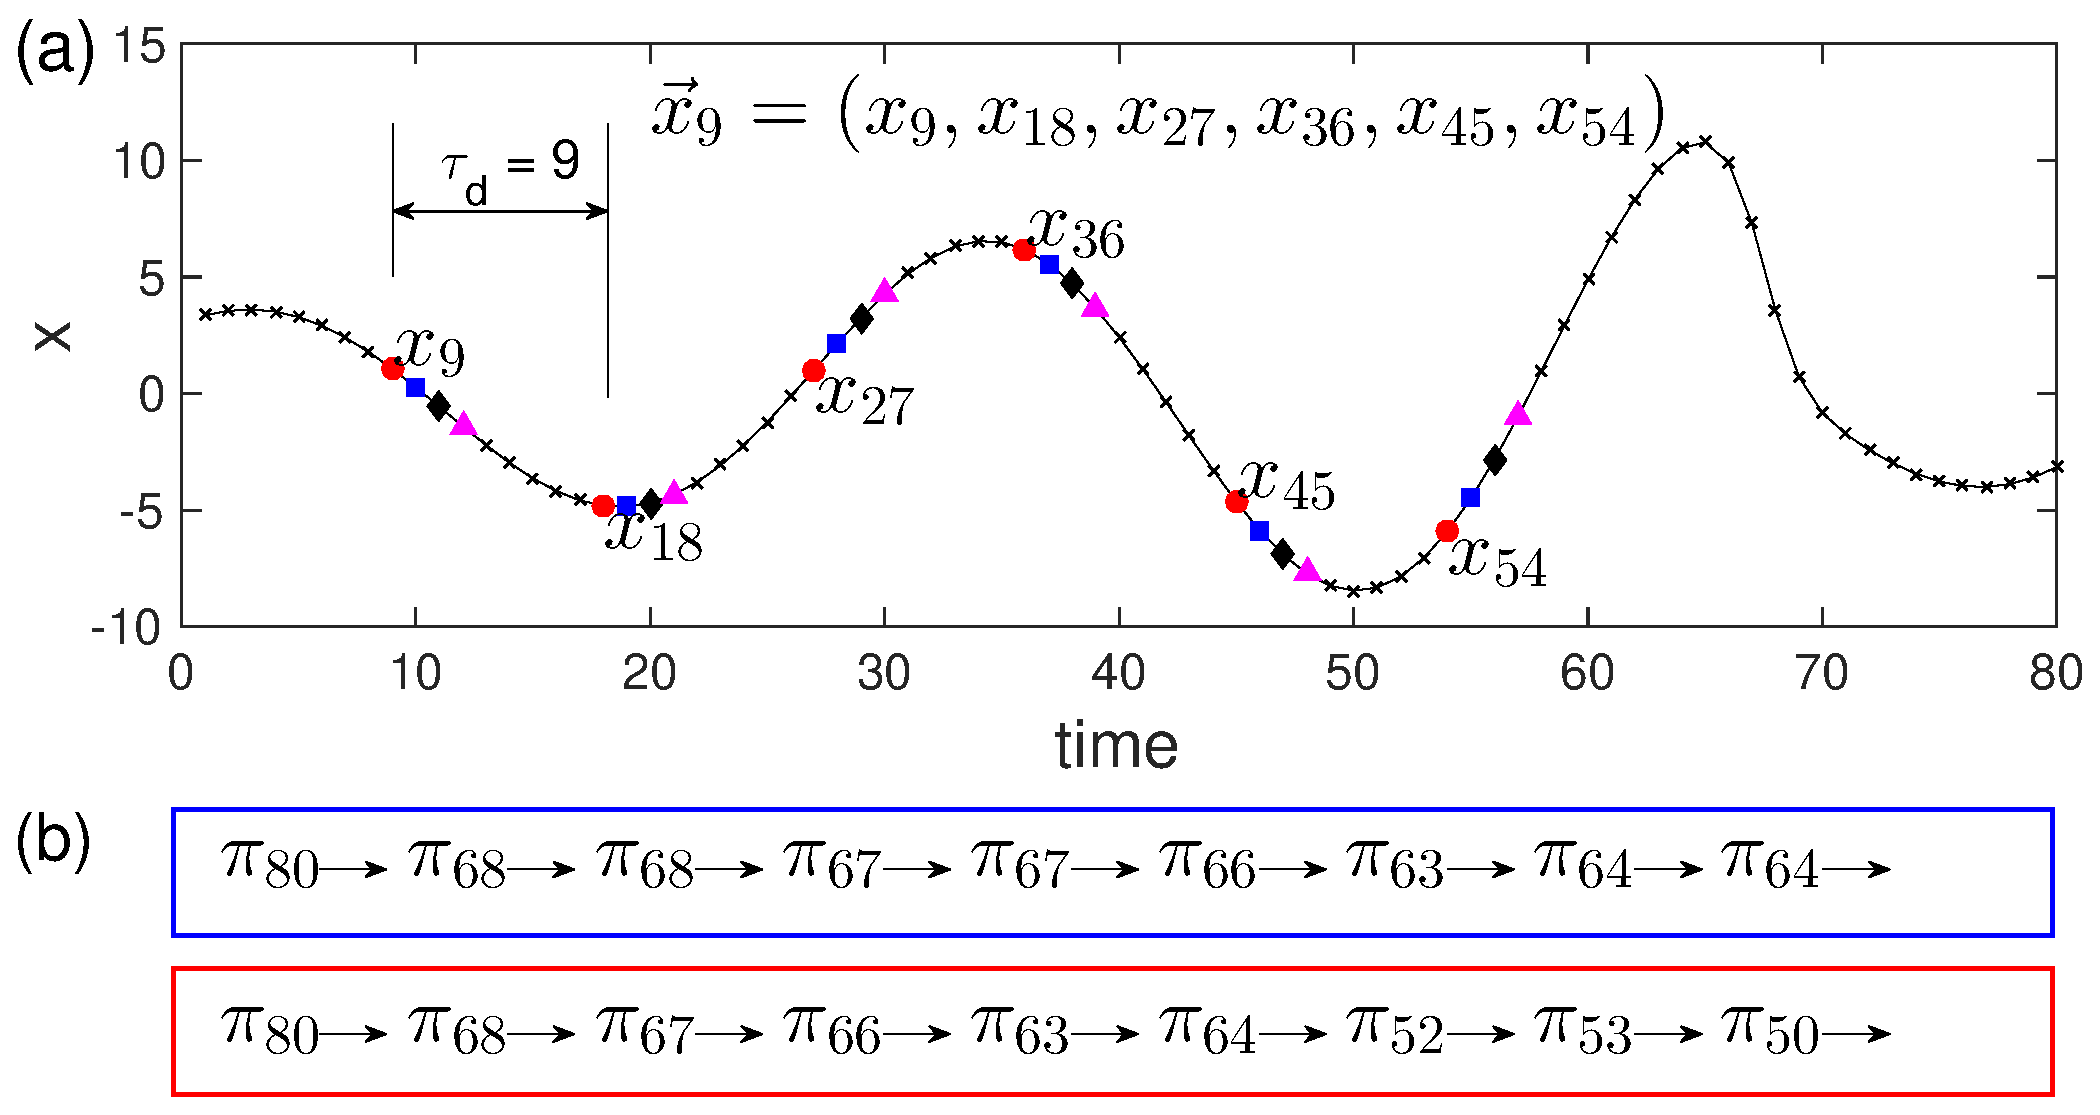
\includegraphics[width=1.3\columnwidth]{timeseriesOPexample.eps}
\caption{(Color online) Illustrative example showing ordinal pattern definitions and evolution. (a) shows an embedding vector $\vec{x}_{9}$ with embedding parameters $\tau_d = 9$ and $D = 6$. (b) The resulting series of ordinal patterns before (top) and after (bottom) removal of all self-transitions. \label{fig:OPexample}}
\end{figure*}

Now, let us transfer the above idea from one to two series of ordinal patterns $\pi_i^{X}$ and $\pi_j^{Y}$ constructed from two possibly interacting systems $X$ and $Y$, respectively, as schematically shown in Fig.~\ref{fig:patternSeriesCond}. For $X$ exhibiting an ordinal pattern $\pi_i$ at some time $t$, we compute the time-lagged co-occurrence frequencies with all ordinal patterns of $Y$ to be observed at time $t+\tau$, i.e., $p(\pi_{j}^{Y}(\tau) | \pi_i^{X})$. When $\tau = 0$, we study the simultaneous co-occurrence of ordinal patterns in both sequences. In turn, non-zero delays $\tau$ capture possible indications of causal relationships among the two systems since it commonly takes some time for the driven process to respond properly to the driving system. An example of $p(\pi_{j}^{Y}(\tau) | \pi_i^{X})$ for two unidirectionally ($X \to Y$) coupled linear stochastic systems \cite{LiPRE2018}
\begin{equation} \label{eq:B}
A: \left \{ \begin{aligned}
x_{t+1} &= -0.3 x_{t} + \varepsilon_t, \\
y_{t+1} &= 0.3 y_{t} - 0.9 x_{t} + \eta_t,
\end{aligned}
\right.
\end{equation}
(with $\{ \varepsilon_t \}$ and $\{ \eta_t \}$ being independent and identically distributed (i.i.d.) Gaussian noises of zero mean and unit variance) with delay $\tau = 1$ is shown in Fig.~\ref{fig:conditionTranOP}. Figure~\ref{fig:conditionTranOP}(a, b) reveals that both cases of $\tau = -1$ and $\tau = 0$ result in rather homogeneous values of $p(\pi_{j}^{Y}(\tau) | \pi_i^{X})$. By contrast, for $\tau=1$, $p(\pi_{j}^{Y}(\tau) | \pi_i^{X})$ presents markedly non-uniform co-occurrence frequencies among the $D!$ ordinal patterns of $Y$ as shown in Fig.~\ref{fig:conditionTranOP}(c). Furthermore, this heterogeneous pattern co-occurrence has been observed for all reference patterns $\pi_i^{X}$ ($i = 1, \dots, D!$) in $X$, as shown in the two-dimensional plots in Fig.~\ref{fig:conditionTranOP}(d-f). More specifically, the heterogeneous time-lagged conditional co-occurrence frequencies of $\pi_j^{Y}$ given the reference pattern $\pi_i^{X}$ for different delays $\tau$ as shown in Fig.~\ref{fig:conditionTranOP}(a-c) are respectively represented by one column in Fig.~\ref{fig:conditionTranOP}(d-f). 

\begin{figure}
	\centering
	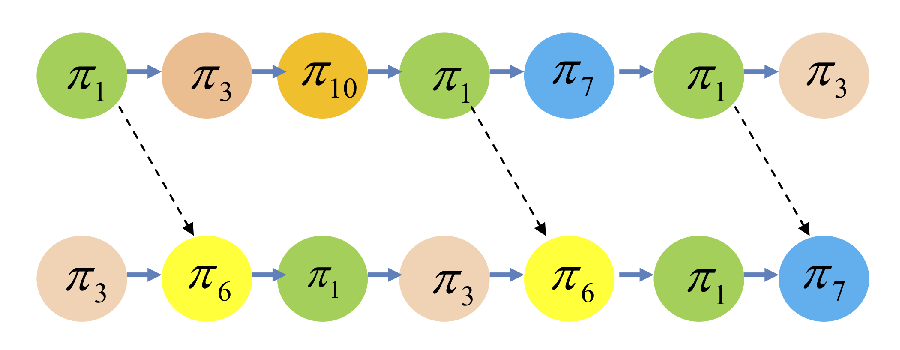
\includegraphics[width=\columnwidth]{patternSeriesCondition.eps}
\caption{(Color online) Schematic illustration of the OPTN analysis for two series of ordinal patterns with a unidirectional coupling $X \to Y$ with a coupling delay of $1$. The time-lagged conditional co-occurrences of the patterns $\pi_i^{X}$ and $\pi_{j}^{Y}(\tau)$ are indicated by dashed arrows. In this example, we observe two cases of occurrences of $\pi_6$ in the $Y$ series when $X$ presents the pattern $\pi_1$ at the previous time step, which is denoted as $\pi_{6}^{Y}(\tau=1) | \pi_{1}$ in the main text.  \label{fig:patternSeriesCond}}
\end{figure}

\begin{figure*}
	\centering
 	\includegraphics[width=2\columnwidth]{cond_allPatterns.eps}
\caption{(Color online) Graph representation of time-lagged conditional co-occurrence frequencies for the ordinal patterns $\pi_{j}(\tau)$ of the $Y$ series when $X$ has the same randomly chosen ordinal pattern $\pi_i^{X}$ for $D = 5$. The pattern $\pi_i^{X}$ is placed in the center while the different patterns $\pi_{j}^{Y}$ are aligned on the unit circle. The thickness of each connecting line corresponds to the time-lagged occurrence frequency of $\pi_j^{Y}$ under the condition that $X$ has pattern $\pi_i^{X}$. Panel (a-c) are for one reference ordinal pattern $\pi_i^{X}$: (a) $p(\pi_{j}^{Y}(\tau=-1) | \pi_{i}^{X}) $, (b) $p(\pi_j^{Y}(\tau=0) | \pi_i^{X})$, and (c) $p(\pi_{j}^{Y}(\tau=1) | \pi_i^{X})$. Panels (d-f) give the corresponding two-dimensional plots for all patterns of $\pi_i^{Y}$ under the condition that $X$ has reference pattern $\pi_i^{X}, i = 1, \dots, D!$. Note that the missing patterns have been indicated by white dots, which are frequently found in the case of $\tau = 1$. The color bar represents the co-occurrence frequencies between patterns. 
\label{fig:conditionTranOP}}
\end{figure*}

From the described construction of OPTNs for the case of two time series, it is obvious that the resulting networks exhibit two distinct types of nodes, corresponding to the ordinal patterns $\pi_i^X$ of $X$ and $\pi_j^Y$ of $Y$, respectively, and exclusively (weighted and directed) links from any $\pi_i^X$ to any $p_j^Y$ based on the corresponding conditional co-occurrence frequencies. Hence, this type of network constitutes a weighted and directed bipartite network. Given that the number of specific network properties tailored to describing the topological characteristics of such networks are rather limited as opposed to unweighted, undirected, and unipartite graphs, in what follows we will introduce a suite of network characteristics that are specifically designed to capture different aspects of the underlying heterogeneity of link weights.

\section{Complexity measures for bipartite OPTNs} \label{sec:measures}

Based on our qualitative observations as shown in Fig.~\ref{fig:conditionTranOP}, in the following we propose a suite of measures to quantitatively characterize the heterogeneous co-occurrence of ordinal patterns in two time series. All these measures will make use of the time-lagged co-occurrence frequencies between ordinal patterns in the two time series under study.

First, we note that for one reference pattern $\pi_i^{X}$ of $X$, the heterogeneity of the \emph{conditional} frequencies of patterns $\pi_{j}^{Y}$ in $Y$ at a time lag $\tau$ can be simply characterized by their corresponding standard deviation
\begin{equation}
\sigma_i^{X} (\tau) = \sqrt{\frac{\sum_{j = 1}^{D!} [p(\pi_{j}^{Y}(\tau) | \pi_i^{X}) - \overline{p(\pi_{j}^{Y}(\tau) | \pi_i^{X})}]^{2} }{D!}}, 
\label{eq:sigmaX}
\end{equation}
where $\overline{\bullet}$ denotes here the average over all patterns $\pi_{j}^{Y}$ in $Y$, i.e., $\overline{p(\pi_{j}^{Y}(\tau) | \pi_i^{X})}$ gives the mean probability of all patterns $\pi_{j}^{Y}(\tau)$ in the series $Y$ to occur at a time-lag $\tau$ under the condition that the series $X$ has exhibited the pattern $\pi_i^{X}$. In the case of no interdependency between $X$ and $Y$, $p(\pi_{j}^{Y}(\tau) | \pi_i^{X})$ will be independent of $\pi_i^{X}$ and, hence, solely reflect the marginal distribution of the ordinal patterns $\pi_j^{Y}$, so that $\overline{p(\pi_{j}^{Y}(\tau) | \pi_i^{X})}=1/D!$ because of the normalization of probabilities. In such a case, any non-zero value of $\sigma_i^{X}$ simply originates from the heterogeneity of the frequency distribution of ordinal patterns in $Y$. If this distribution is homogeneous, the numerator of Eq.~\eqref{eq:sigmaX} will be (close to) zero. In turn, if there is dependency between $Y$ and $X$, $\overline{p(\pi_{j}^{Y}(\tau) | \pi_i^{X})}\neq 1/D!$ and, hence, $\sigma_i^{X}(\tau)$ will differ from the aforementioned benchmark (independence) case. Hence, any significant deviation of $\sigma_i^{X}(\tau)$ from this benchmark, which can be computed by replacing in Eq.~\eqref{eq:sigmaX} $\overline{p(\pi_{j}^{Y}(\tau) | \pi_i^{X})}$ by $\pi_j^{Y}$, will indicate the presence of (time-lagged) coupling between both systems in the (causal) sense of $X$ determining the behavior of $Y$.

While the above considerations have focused on a single ordinal pattern $\pi_i^{X}$ in $X$ only, we obtain a general measure for the corresponding dependency between $X$ and $Y$ by summing up the values found for all ordinal patterns $\pi_i^{X}$ as
\begin{equation}
\sigma_{X\to Y} (\tau) = \sum_{i=1}^{D!} \sigma_{i}^{X} (\tau). 
\end{equation}

Our second characteristic property is based on a similar rationale as a measure recently proposed in ref.~\cite{McCullough2017b}. Here, we first quantify the local ordinal pattern (node-wise) co-occurrence by the Shannon entropy
\begin{equation} \label{eq:localH}
H_{X \to Y}^{\pi_i}(\tau) = - \sum_{j=1}^{D!} p(\pi_{j}^{Y}(\tau) | \pi_i^{X}) \log_2 p(\pi_{j}^{Y}(\tau) | \pi_i^{X}), 
\end{equation}
where the summation runs over all possible patterns of $\pi_j^{Y}(\tau)$. Note that for each pattern $\pi_i^{X}$ and delay $\tau$, a normalization is introduced by $\sum_{j=1}^{D!} p(\pi_{j}^{Y}(\tau) | \pi_i^{X}) = 1$. Since patterns $\pi_i$ can have different empirical frequencies $p(\pi_i^{X})$, we further compute the expectation value of the co-occurrence entropy of the whole bipartite OPTN as 
\begin{equation}  \label{eq:globalH}
H_{X \to Y}(\tau) = \sum_{i=1}^{D!} p(\pi_i^{X}) H_{X \to Y}^{\pi_i}(\tau), 
\end{equation}
which we call global ordinal pattern co-occurrence entropy. 

For a memoryless and stationary stochastic process, we may expect $p(\pi_i^{X} )= \frac{1}{D!}$ for any pattern order $D$. Accordingly, the local (per-node) co-occurrence entropy of Eq. \eqref{eq:localH} simplifies as 
\begin{equation}
p(\pi_{j}^{Y}(\tau) | \pi_i^{X}) \log_2 p(\pi_{j}^{Y}(\tau) | \pi_i^{X}) = \frac{1}{D!} \log_2 \frac{1}{D!}. 
\end{equation}
Therefore, the global co-occurrence entropy (Eq.~\eqref{eq:globalH}) has a maximal value $H_{X \to Y} = \log_2 D!$ if all $D!$ patterns are distributed uniformly in both, $X$ and $Y$. For example, $H_{X \to Y} \approx 6.9$ when $D = 6$ for two series of ordinal patterns that are obtained from two independent identically distributed noise processes. We note that this observation might be used for obtaining a proper re-normalization of $H_{X \to Y}(\tau)$, which shall however not further pursued here.

Finally, we propose a third measure to capture possible causal influences of $X$ on $Y$, which quantifies how much more heterogeneous the co-occurrence frequencies $p(\pi_{j}^{Y} | \pi_i^{X})$ are in comparison with the marginal distribution $p(\pi_j^{Y})$ (without prior knowledge of the driving process). For this purpose, we compute the node-wise Kullback-Leibler divergence (KLD) in the following way: 
\begin{equation} \label{eq:localKLD}
\text{KLD}^{\pi_i}(\tau) = \sum_{j=1}^{D!} p(\pi_{j}^{Y}(\tau) | \pi_i^{X}) \log_2 \frac{p(\pi_{j}^{Y}(\tau) | \pi_i^{X})}{p(\pi_j^{Y})}, 
\end{equation}
which appears to be closer to the Granger-type (predictive) idea of causality than the two previous measures. Here, we use the KLD to distinguish between two probability distributions $p(\pi_{j}^{Y} | \pi_i^{X})$ and $p(\pi_j^{Y})$, the value of which vanishes if and only if the ordinal pattern series $\{\pi_i^{X}\}$ and $\{\pi_j^{Y}\}$ are independent, while any positive value suggests a possible directed influence from $X$ to $Y$. As a corresponding global characteristic, the expected KLD of the whole network is calculated as
\begin{equation}  \label{eq:globalKLD} 
\text{KLD}_{X \to Y}(\tau) = \sum_{i=1}^{D!} p(\pi_i^{X}) \text{KLD}^{\pi_i}(\tau), \
\end{equation}
where the summation runs over all patterns $\pi_i^{X}$ of $X$. 

{\color{red} We note that the computation of $H_{X\to Y}(\tau)$ is similar with that has been proposed in  \cite{LiNI2010}, while the KLD is similar with the symbolic transfer entropy \cite{Staniek2008}. The main difference is the parameter $\tau$.  In \cite{Staniek2008}, $\tau$ is treated as an algorithmic parameter which had been suggested as $\tau = 1$. Furthermore, it has been assumed that the empirical choice of $\tau = 1$ is always applicable if a meaningful natural sampling rate of time series is a available. From the descriptions above, it is clear that our method interprets $\tau$ differently, considering to extract the proper coupling delay $\tau$ explicitly by treating it as a dynamical unknown variable. }

\section{Numerical examples} \label{sec:res}
In this section, we demonstrate that the time-lagged ordinal pattern co-occurrence complexity measures introduced in the previous section can capture causal interactions in both, unidirectional and bidirectional coupling configurations. In order to illustrate this, we consider examples from two typical classes of time-discrete dynamical systems: simple stochastic processes and chaotic maps. 

\subsection{Coupled stochastic processes} \label{sec:GCs}
We first test our measures regarding their capability to correctly identify coupling directions and delays among simple one-dimensional stochastic processes. For this purpose, we study two examples in a unidirectional coupling configuration and two others in a bidirectional setting. Moreover, we consider cases with a single delay term versus such with more than one delay, as well as nonlinear model versions obtained by static nonlinear transformations of the first subsystem as proposed in ref.~\cite{LiPRE2018}.

In all considered models, we generate time series $\{ x_t \}$ and $\{ y_t \}$ of length $N=10^{5}$, which are then used to construct ordinal pattern representations with the embedding parameters $D = 5$ and $\tau_d = 100$. We have checked that our results do not change qualitatively if other parameter combinations are chosen (not shown). The relevance of all inferred interaction delays has been confirmed by switching the roles of $X$ and $Y$ (for instance, a positive delay $\tau$ from $X$ to $Y$ should coincide with a negative delay $-\tau$ when exchanging the two systems). The results presented in the following are based on averages over 20 independent realizations of the considered processes. {\color{red}The deviation of the results from this ensemble of realizations is neglect-able and error bars are tiny (not shown). }

\subsubsection{Unidirectional coupling}

We start with the system of two coupled linear stochastic systems from Eq.~\eqref{eq:B}. A nonlinear transformation $f(x) = \left[\frac{x + | x |}{2}\right]^{5}$ is applied to each realization of the first system $X$, and the resulting realization of the transformed system $\tilde{X}$ is denoted as $\{\tilde{x}_t\}$. 

Based on the resulting sequences of ordinal patterns, we compute the three measures $\sigma_{X \to Y}(\tau)$, $H_{X \to Y}(\tau)$ and $\text{KLD}(\tau)$ and show the corresponding results in Fig.~\ref{fig:stdHeqB}. We clearly find at $\tau = 1$ a unique maximum of $\sigma_{X \to Y}(\tau)$ and $\text{KLD}(\tau)$ (Fig.~\ref{fig:stdHeqB}(a,e)) while $H_{X\to Y}(\tau)$ presents a minimum (Fig.~\ref{fig:stdHeqB}(c)). Thus, all three measures consistently suggest that there is an interaction from $X$ to $Y$ at a delay $\tau = 1$. Almost identical results are obtained if the system $X$ is replaced by its nonlinearly transformed counterpart $\tilde{X}$ (Fig.~\ref{fig:stdHeqB}(b,d,f)). 

\begin{figure}
	\centering
	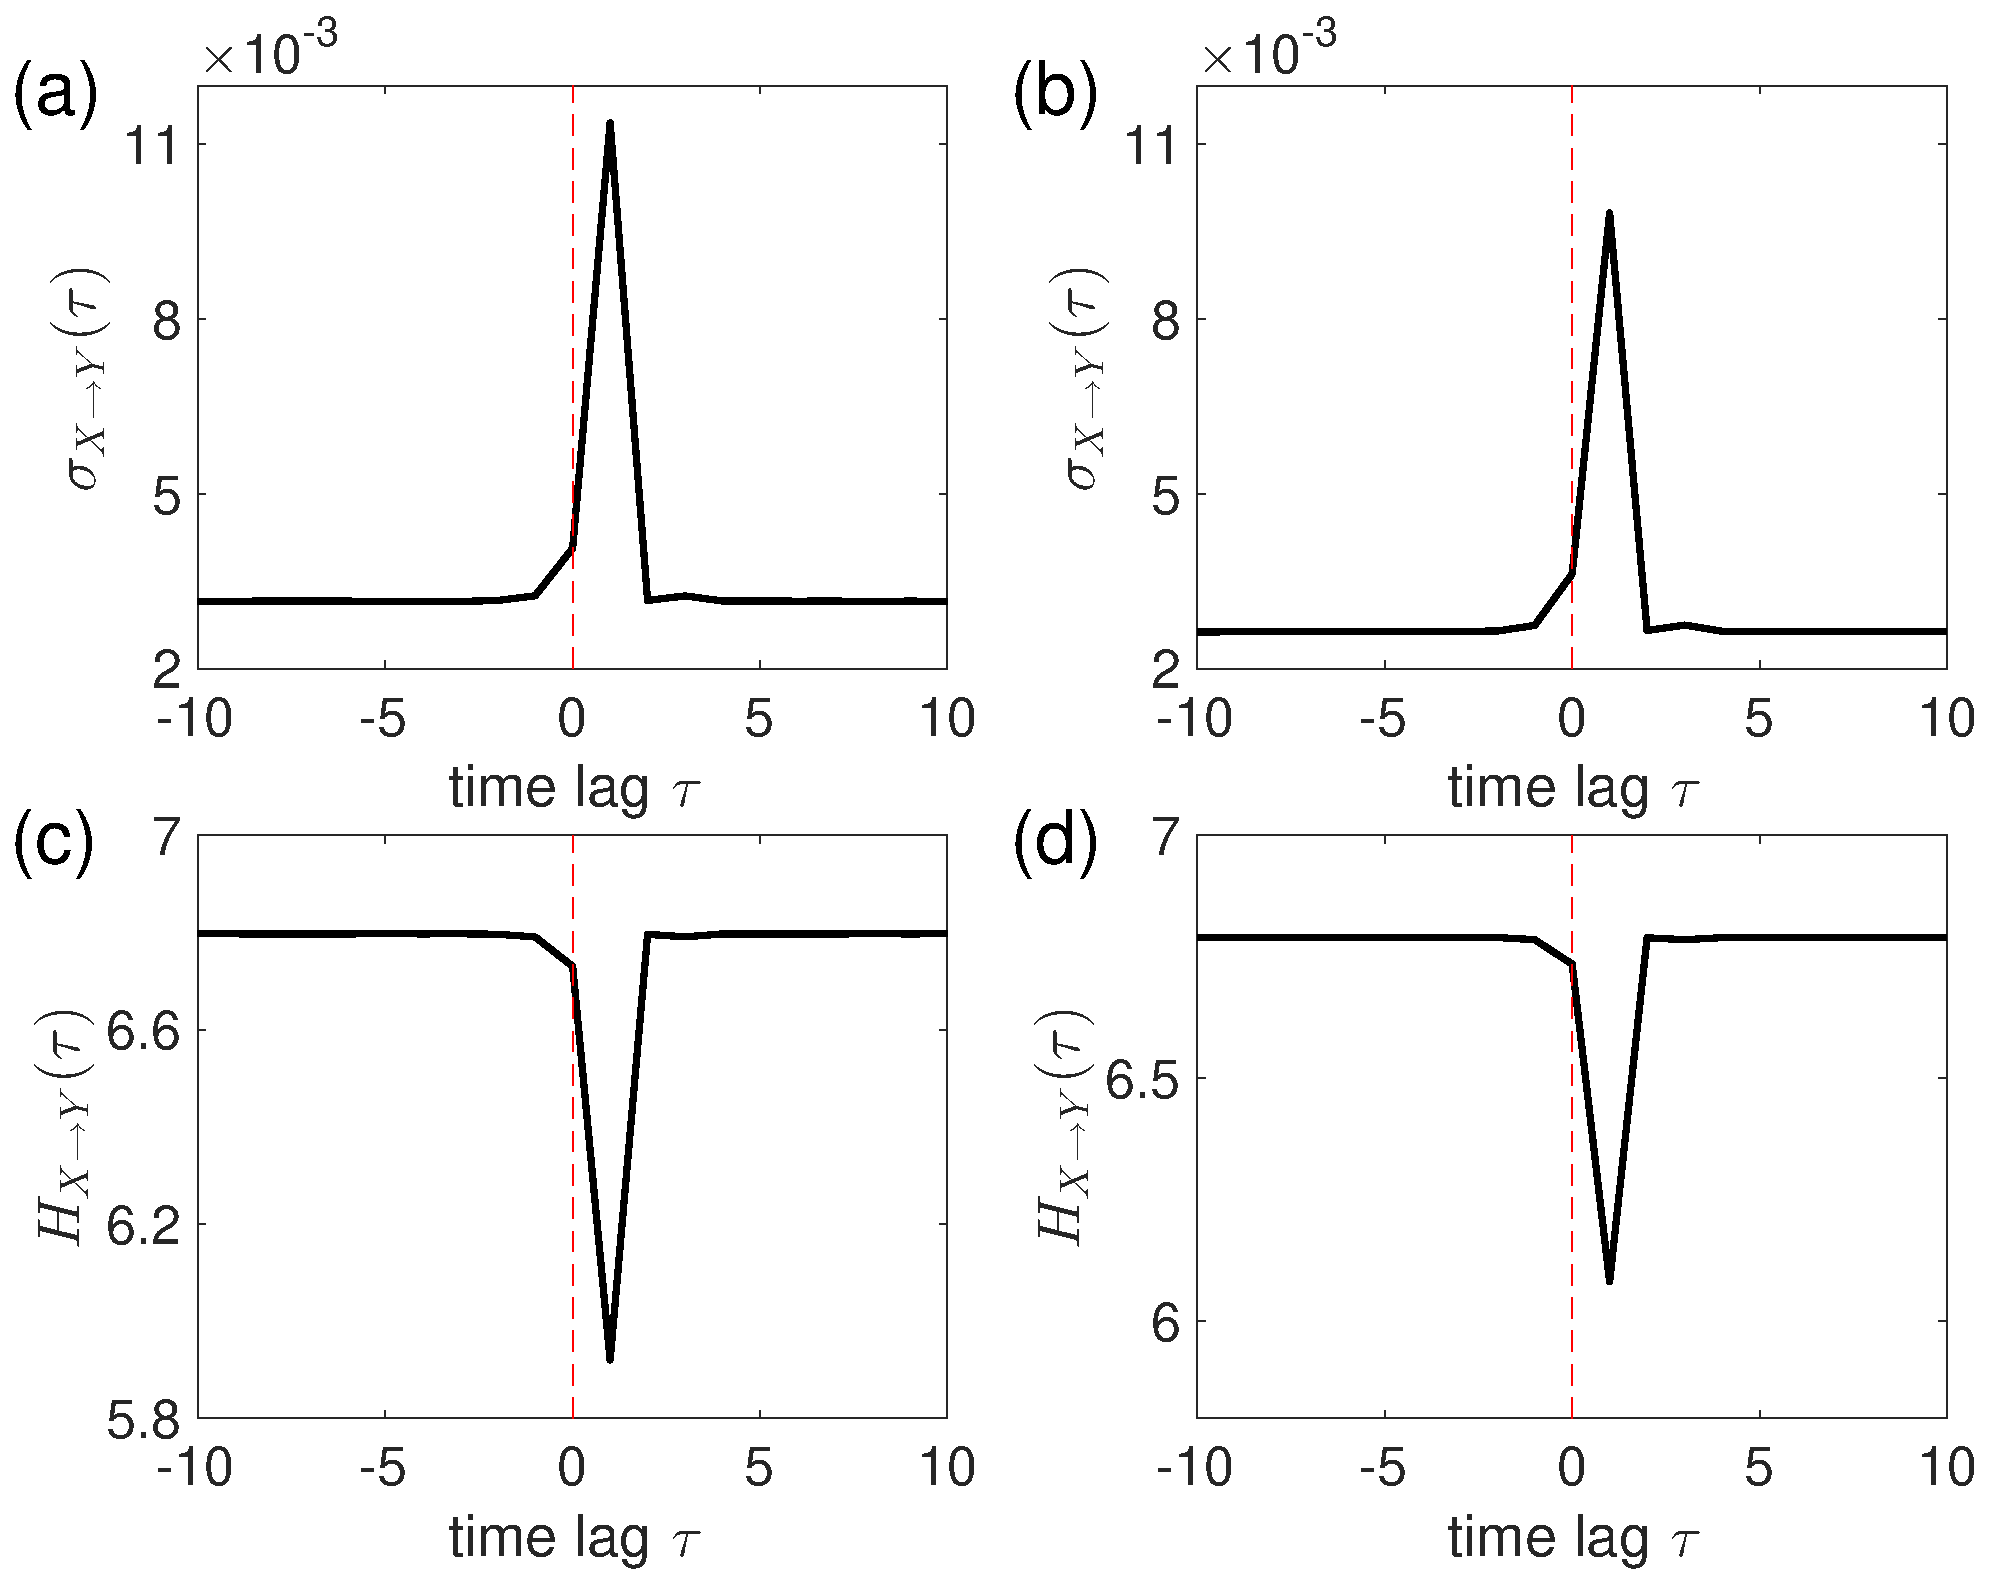
\includegraphics[width=\columnwidth]{E_B.eps}
	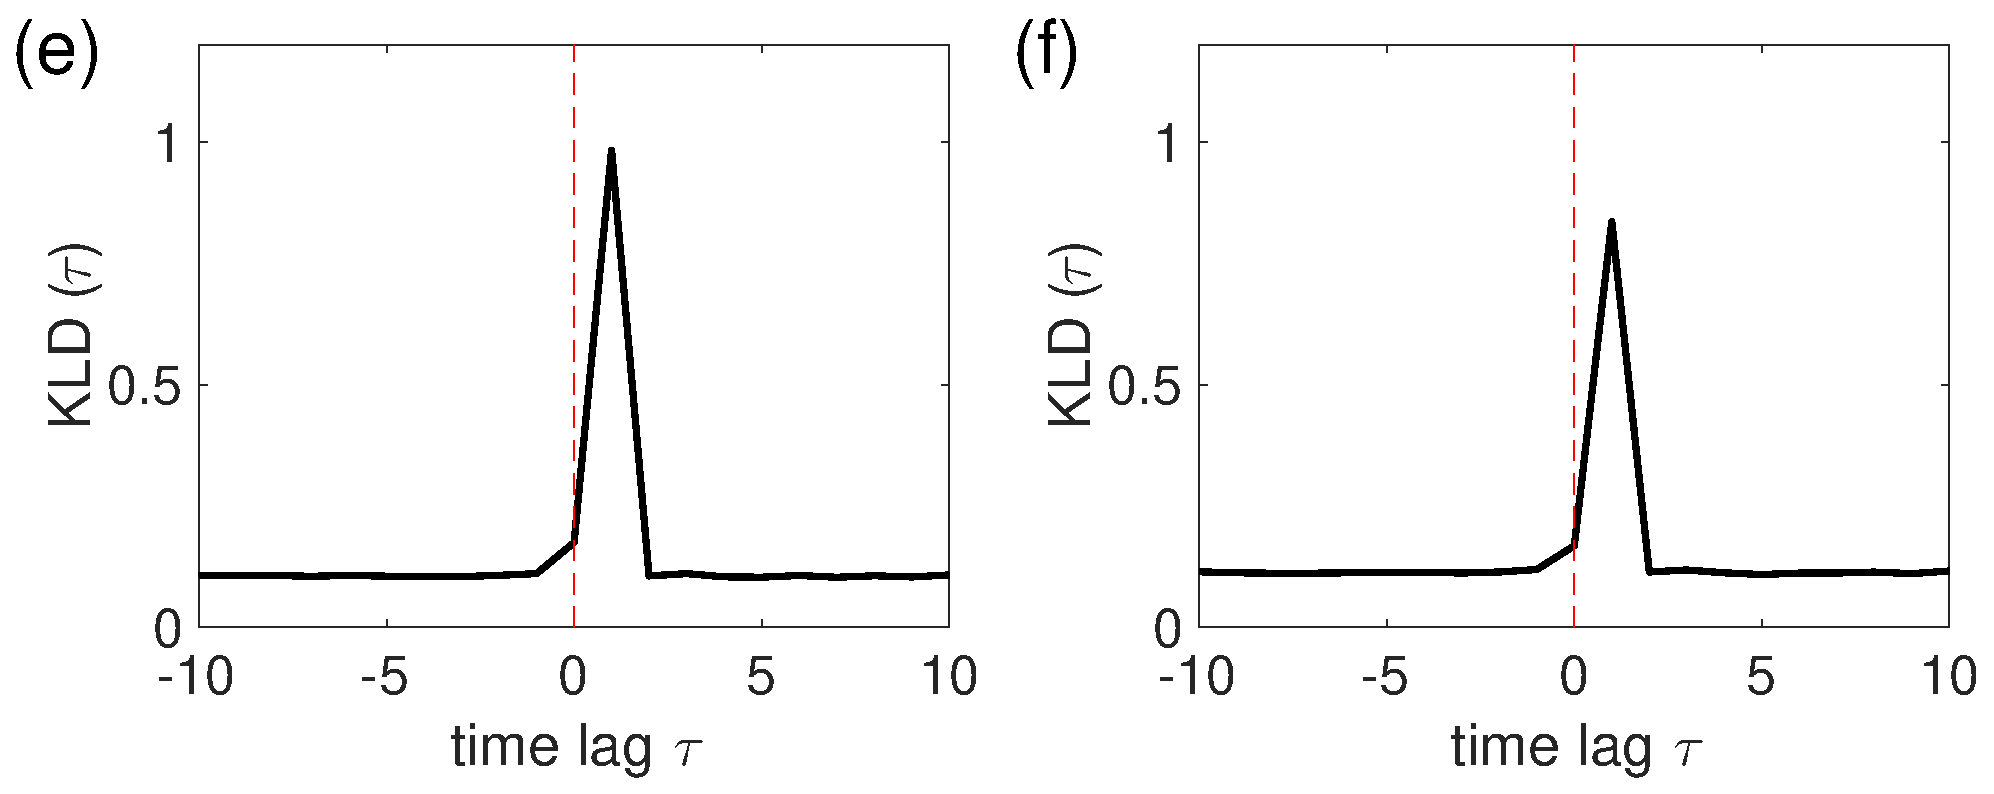
\includegraphics[width=\columnwidth]{KL_B.eps}
\caption{(Color online) Values of three ordinal pattern co-occurrence complexity measures in dependence on the mutual delay $\tau$ for realizations of Eq.~\eqref{eq:B}: (a,b) $\sigma_{X\to Y}(\tau)$, (c,d) $H_{X \to Y}(\tau)$, (e,f) $\text{KLD}(\tau)$. (a,c,e) show the results for realizations from the linear model, while (b,d,f) correspond to the nonlinear transformation of the first subsystem as described in the text. The vertical red dashed lines indicate the values for vanishing mutual delay ($\tau=0$).
\label{fig:stdHeqB}}
\end{figure}

When introducing more interaction delays from $X$ to $Y$, $\sigma_{X\to Y}(\tau)$, $H_{X \to Y}(\tau)$ and $\text{KLD}(\tau)$ exhibit additional maxima and minima, respectively, at various values of $\tau$. To illustrate this, we generate time series from the following linear system~\cite{LiPRE2018}:
\begin{equation} \label{eq:C}
B: \left \{ \begin{aligned}
x_{t+1} &= - \sum_{k=0}^{7} c_k x_{t-k} + \varepsilon_t, \\
y_{t+1} &= - \sum_{k=0}^{7} c_k y_{t-k} + 100 \sum_{k=0}^{8} c_k x_{t-k} + \eta_t,
\end{aligned}
\right.
\end{equation}
where $\varepsilon_t$ and $\eta_t$ are again independent Gaussian random variables. In this model, there are nine interaction terms from $X$ to $Y$ at different delays. By taking the coefficients $\{ c_k \}$ from the polynomial $\sum_{k=0}^{8} c_k z^{k} = [(1 - r e^{-2\pi i f}z)(1 - r e^{2\pi i f} z)]^{4}$ with $f = 0.1$ and $r = 0.8$~\cite{LiPRE2018}, it is ensured that the evolution of $Y$ is influenced more by the interaction terms at smaller delays than those with larger delays. A nonlinearly transformed signal $\tilde{X}$ is obtained by setting $\tilde{x}_{t} = x_{t}^{5}$. 

In comparison with the previous case of a system with only one interaction delay $\tau$ (Fig.~\ref{fig:stdHeqB}), the presence of multiple interaction delays is clearly identified by all three measures (Fig.~\ref{fig:stdHeqC}). However, since these interactions occur at subsequent delays, the corresponding effects partially cancel each other, resulting in a succession of local maxima and minima of these measures. Hence, not all individual delays are identified by our approach in the considered setting. Notably, the nonlinearly transformed version of the model shows again results that are almost equivalent to those of the underlying linear version.

\begin{figure}
	\centering
	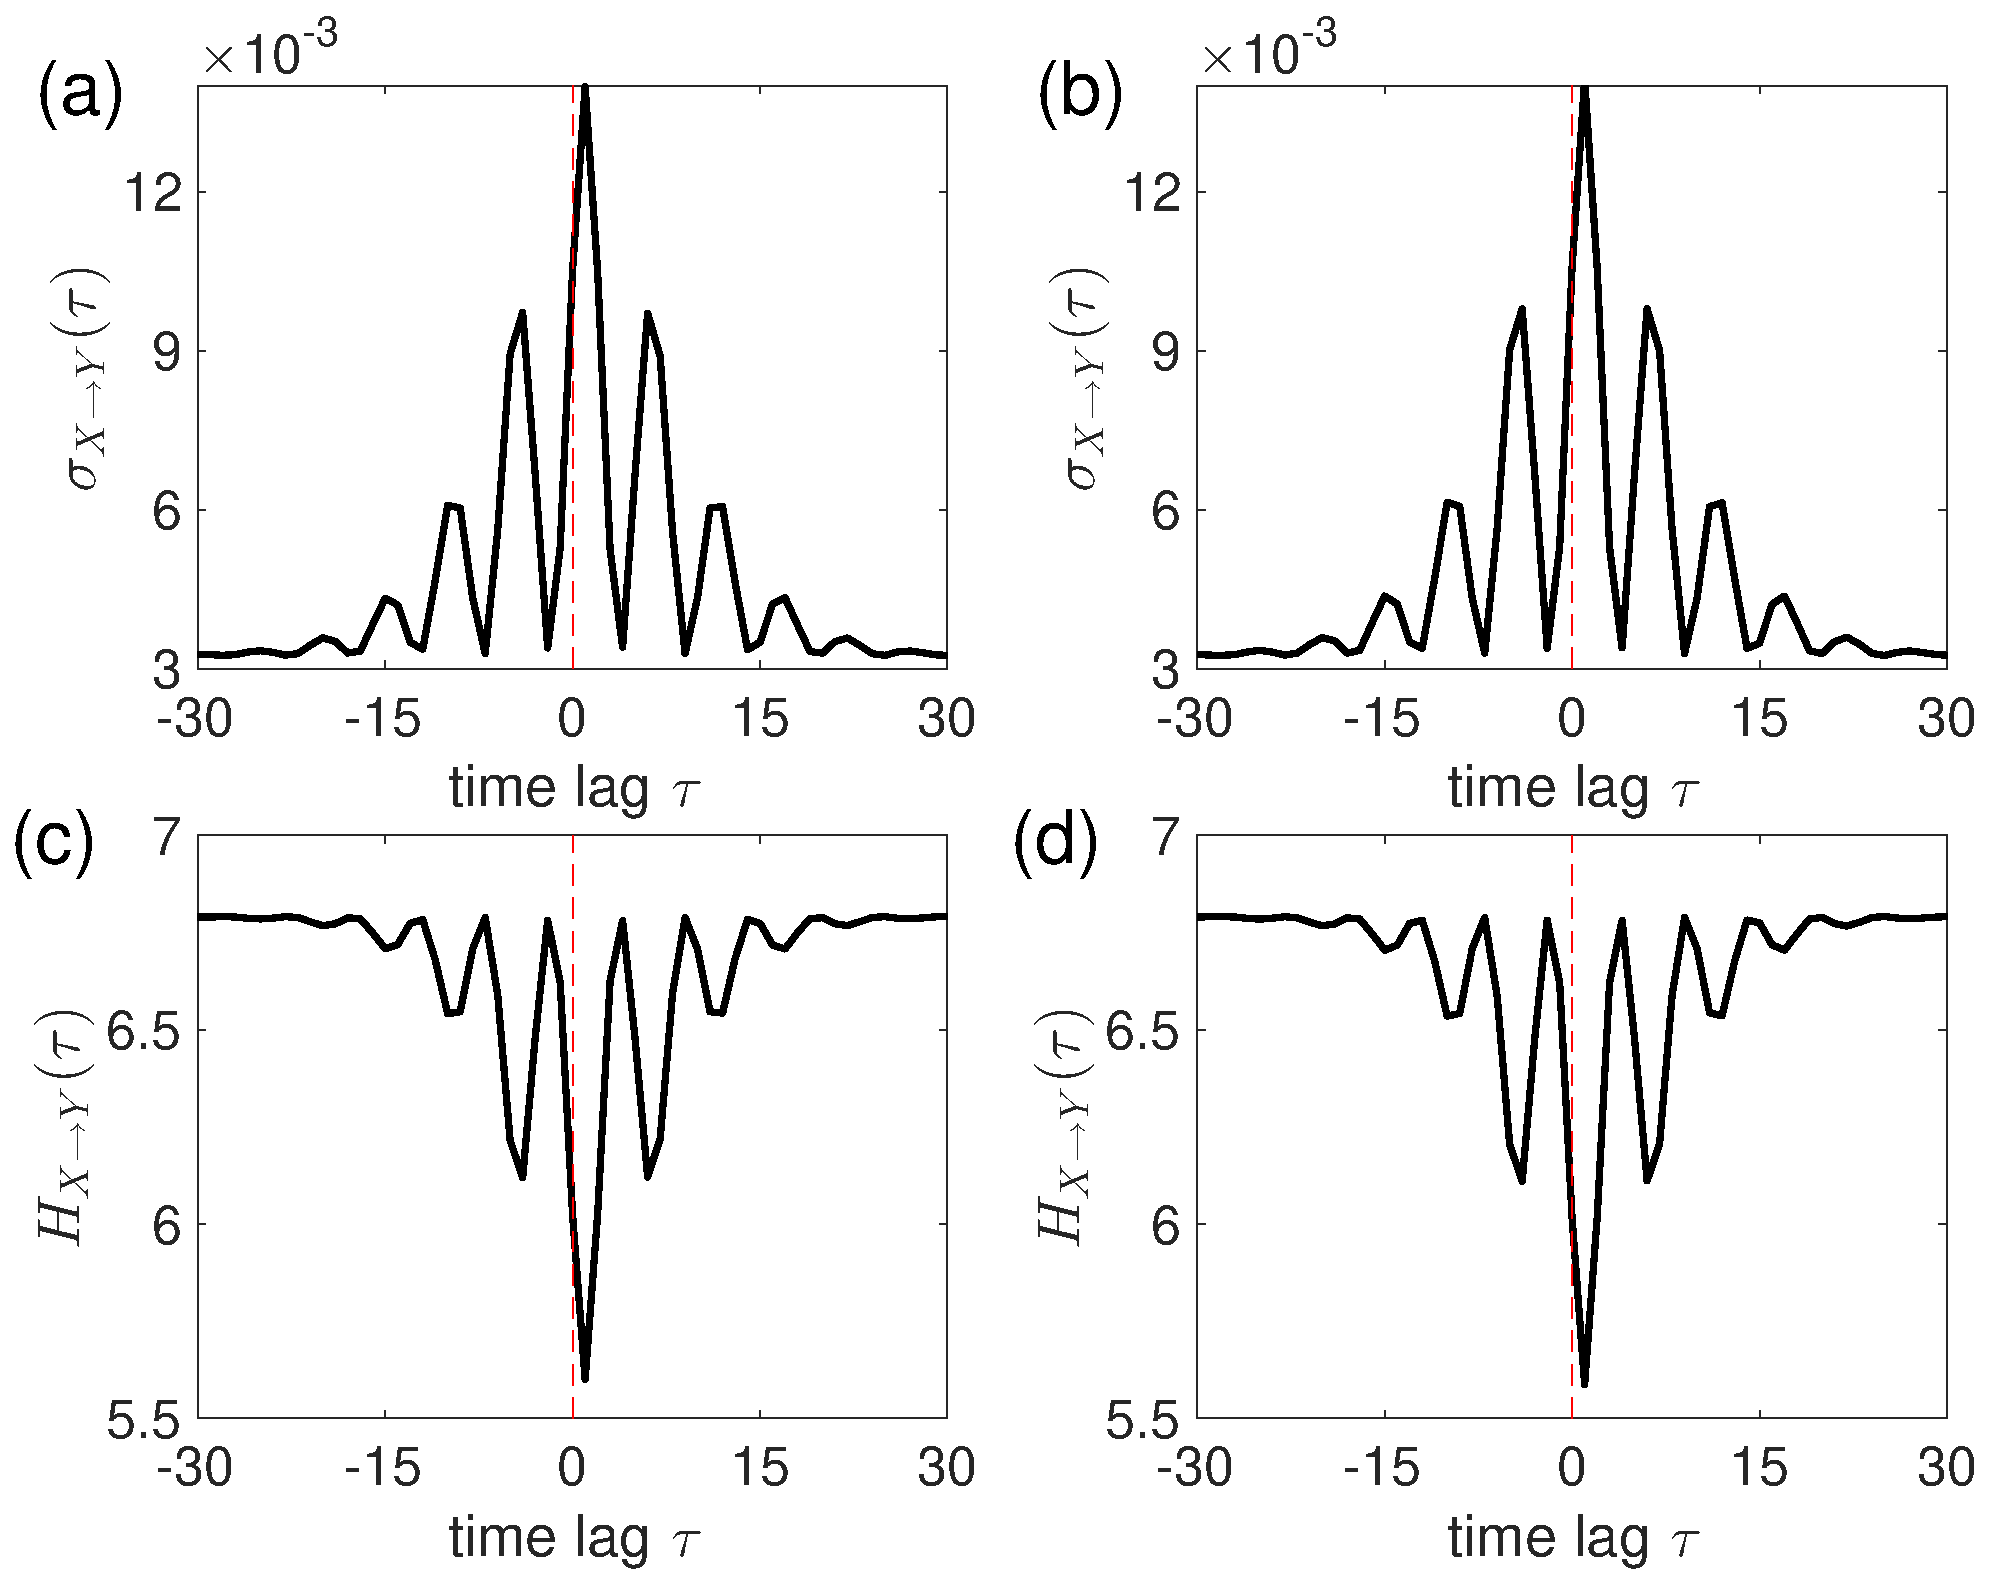
\includegraphics[width=\columnwidth]{E_C.eps}
	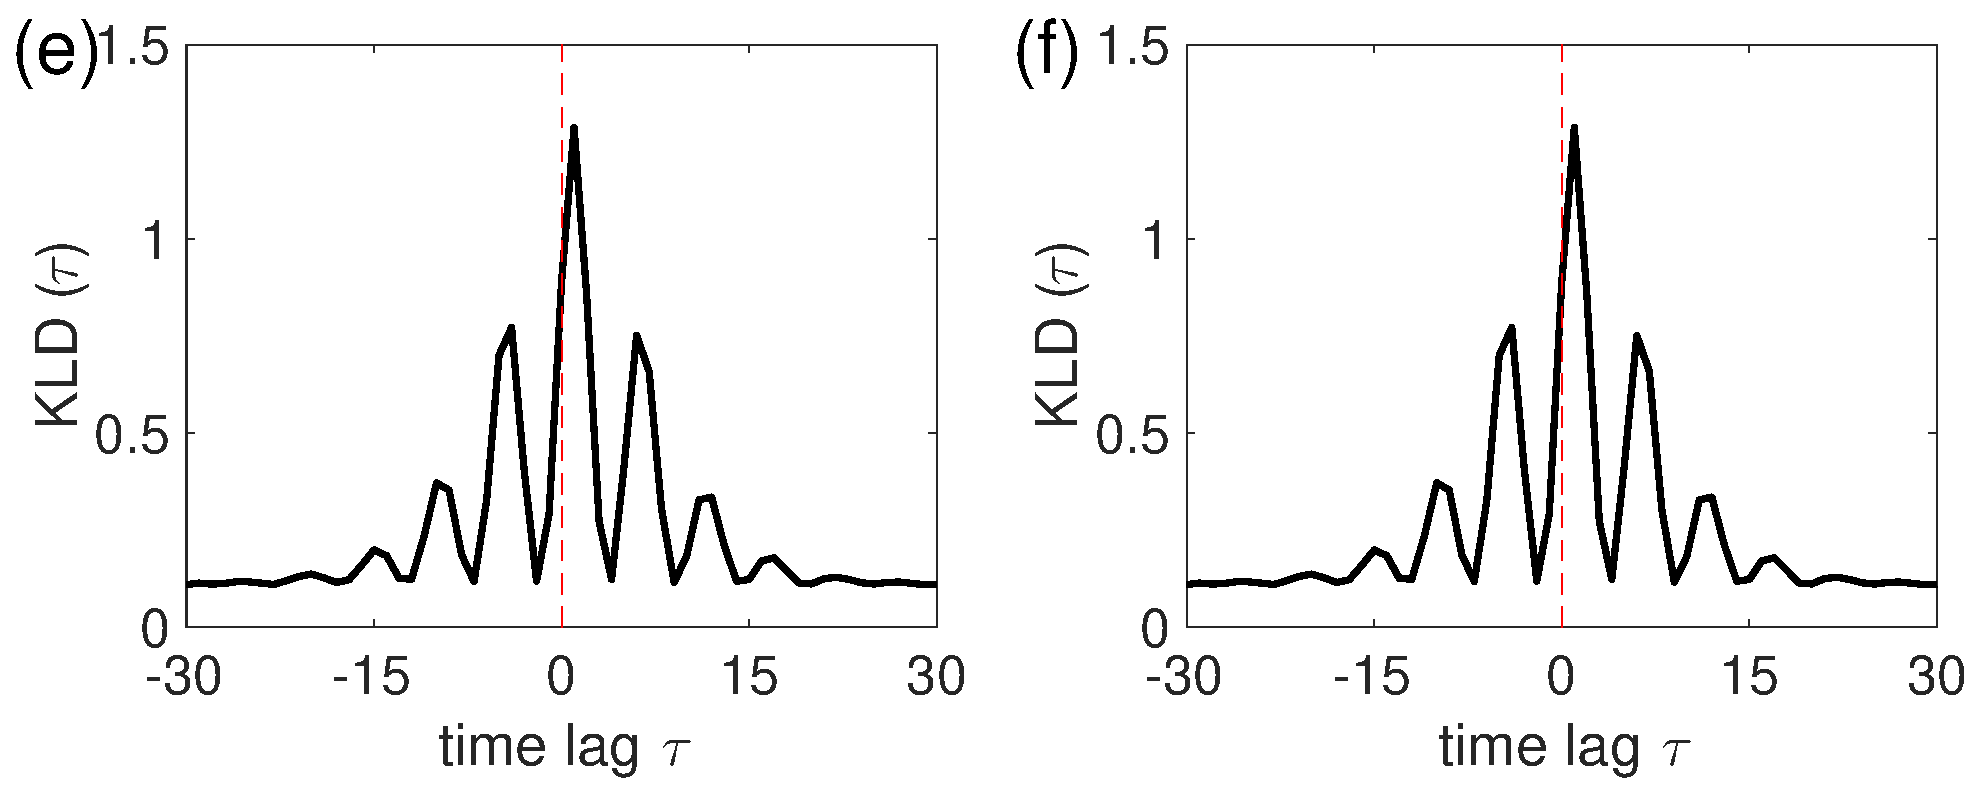
\includegraphics[width=\columnwidth]{KL_C.eps}
\caption{(Color online) Same as in Fig.~\ref{fig:stdHeqB} but for Eq.~\eqref{eq:C}.  \label{fig:stdHeqC}}
\end{figure}

\subsubsection{Bidirectional coupling}

Next, we consider a symmetric bidirectional interaction with a delay of $\tau = 1$ from $X$ to $Y$ and from $Y$ to $X$. The corresponding numerical model reads as follows: 
\begin{equation} \label{eq:D}
C: \left \{ \begin{aligned}
x_{t+1} &= - 0.5 y_{t} + \varepsilon_t, \\
y_{t+1} &= - 0.5 x_{t} + \eta_t, 
\end{aligned}
\right.
\end{equation}
where $\{ \varepsilon_t \}$ and $\{ \eta_t \}$ are again i.i.d standard Gaussian random variables. The nonlinearly transformed signal $\tilde{X}$ is obtained by $\tilde{x}_{t} = x_{t}^{2}$. In this case, $X$ influences $Y$ at a delay $\tau = 1$ while $Y$ influences $X$ at the same delay. As shown in Fig.~\ref{fig:stdHeqD}(a,c,e), both delays are correctly identified by $\sigma_{X \to Y}(\tau)$, $H_{X \to Y}(\tau)$ and $\text{KLD}(\tau)$. For the nonlinearly transformed case, this result is essentially reproduced. In all cases, the corresponding measures exhibit two large peaks/troughs at the positive time lag $\tau = 1$ and the negative time delay $\tau = -1 $. This indicates that the employed coupling is bidirectional and symmetric in both the linear and nonlinear systems. 

\begin{figure}
	\centering
	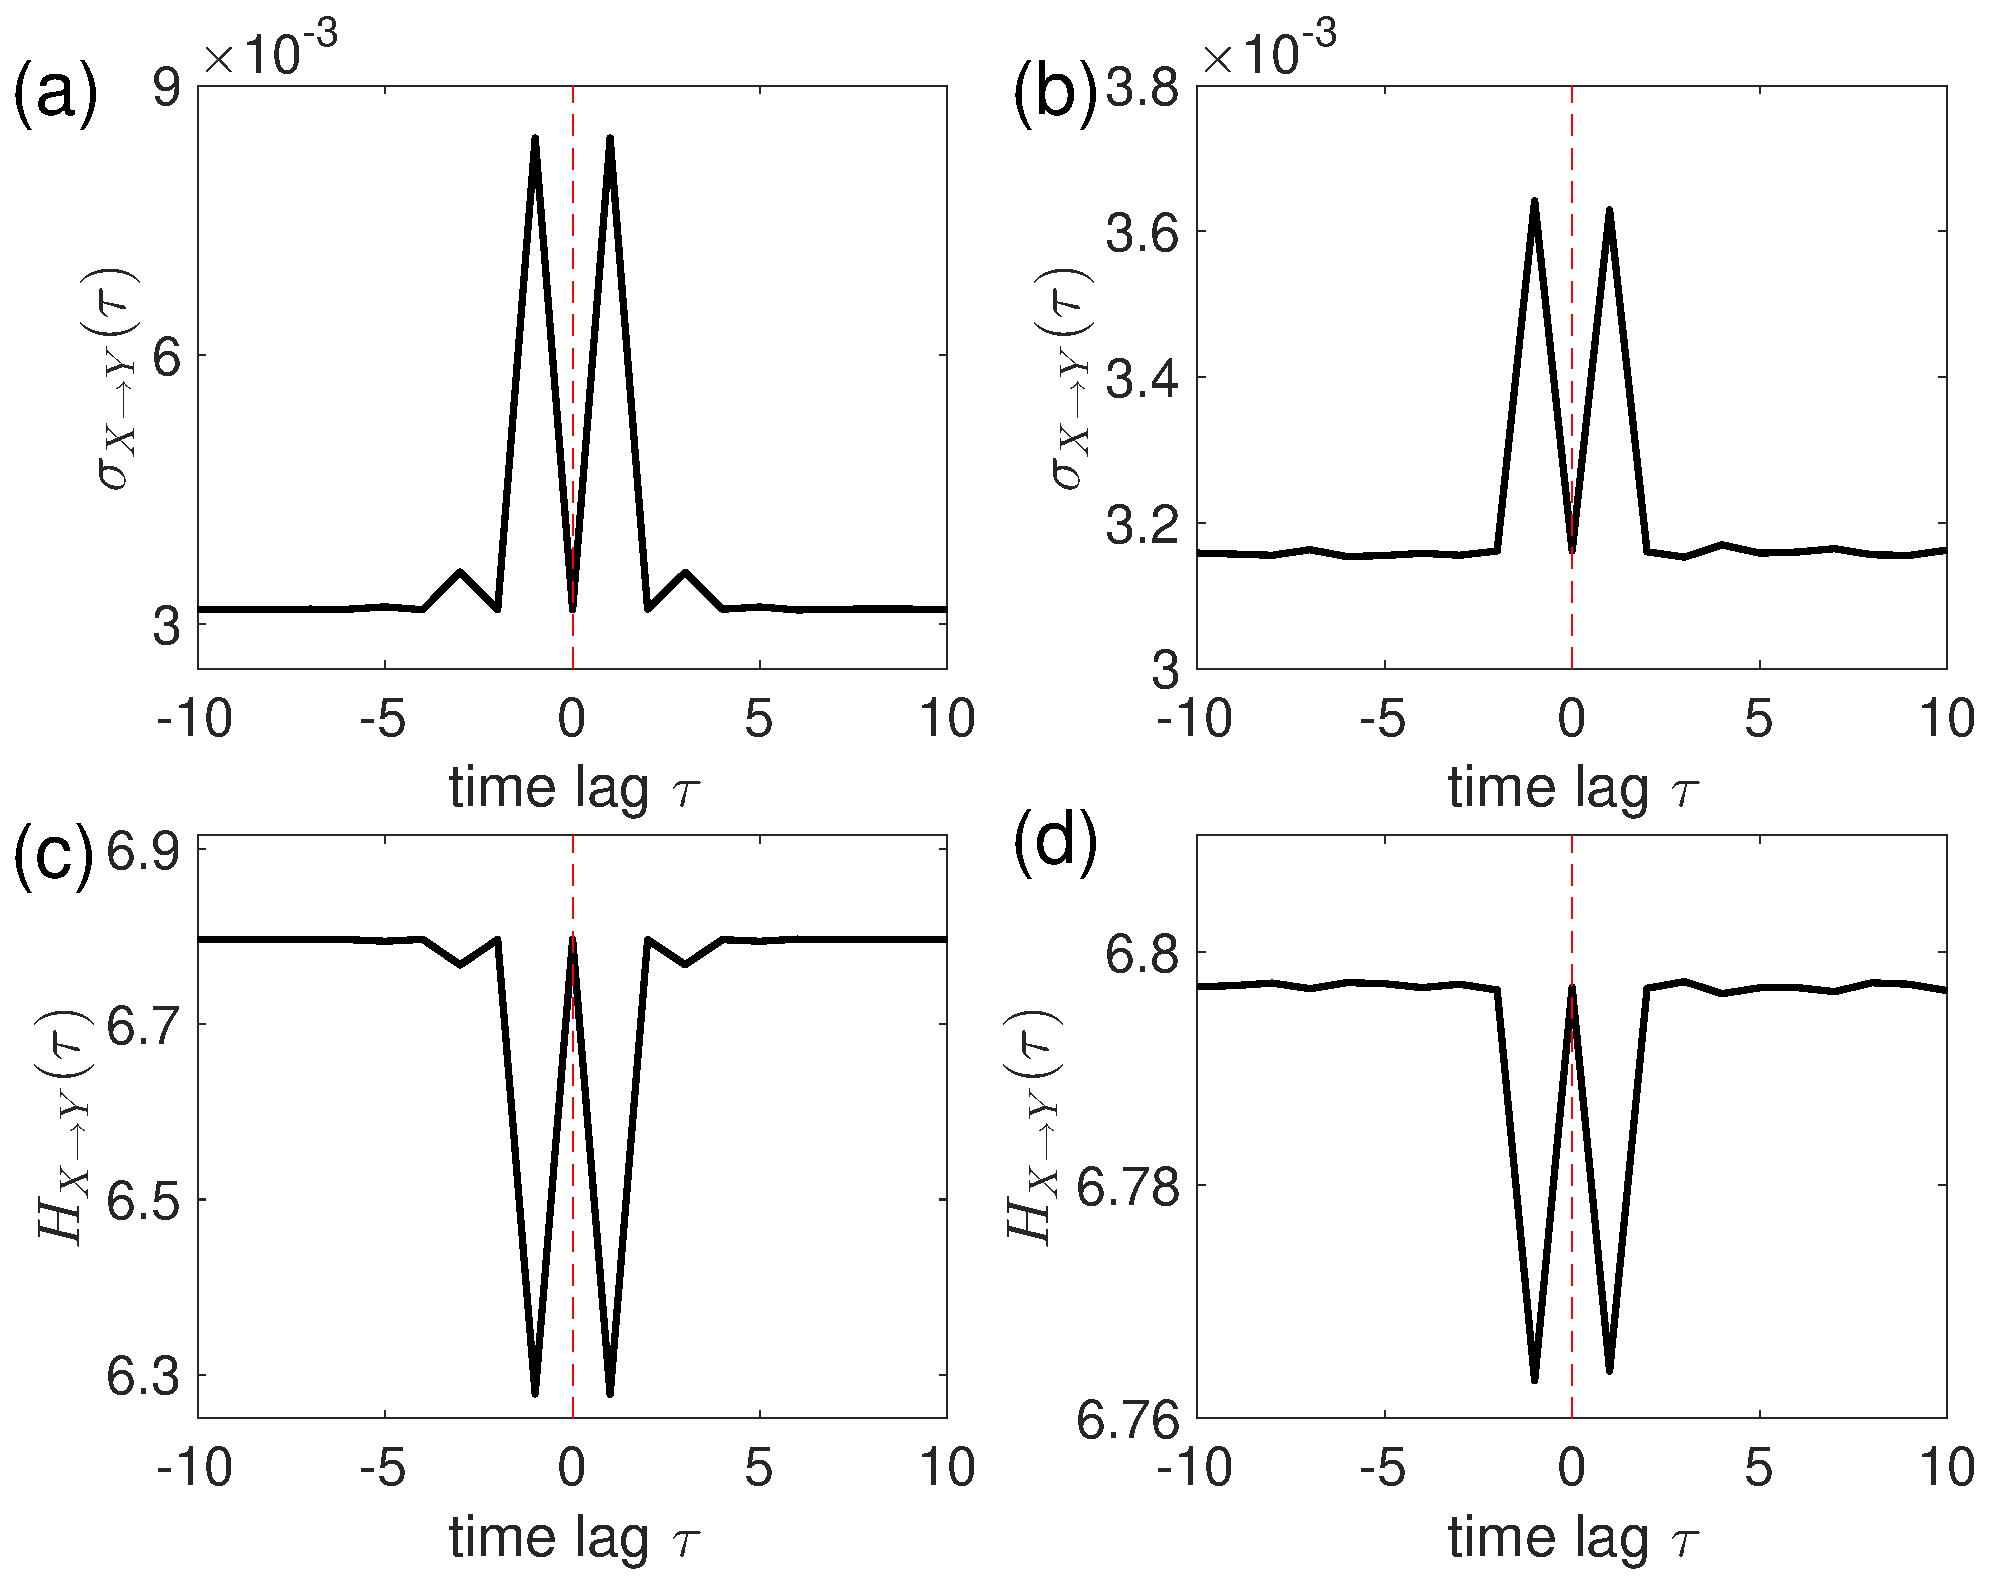
\includegraphics[width=\columnwidth]{E_D.eps}
	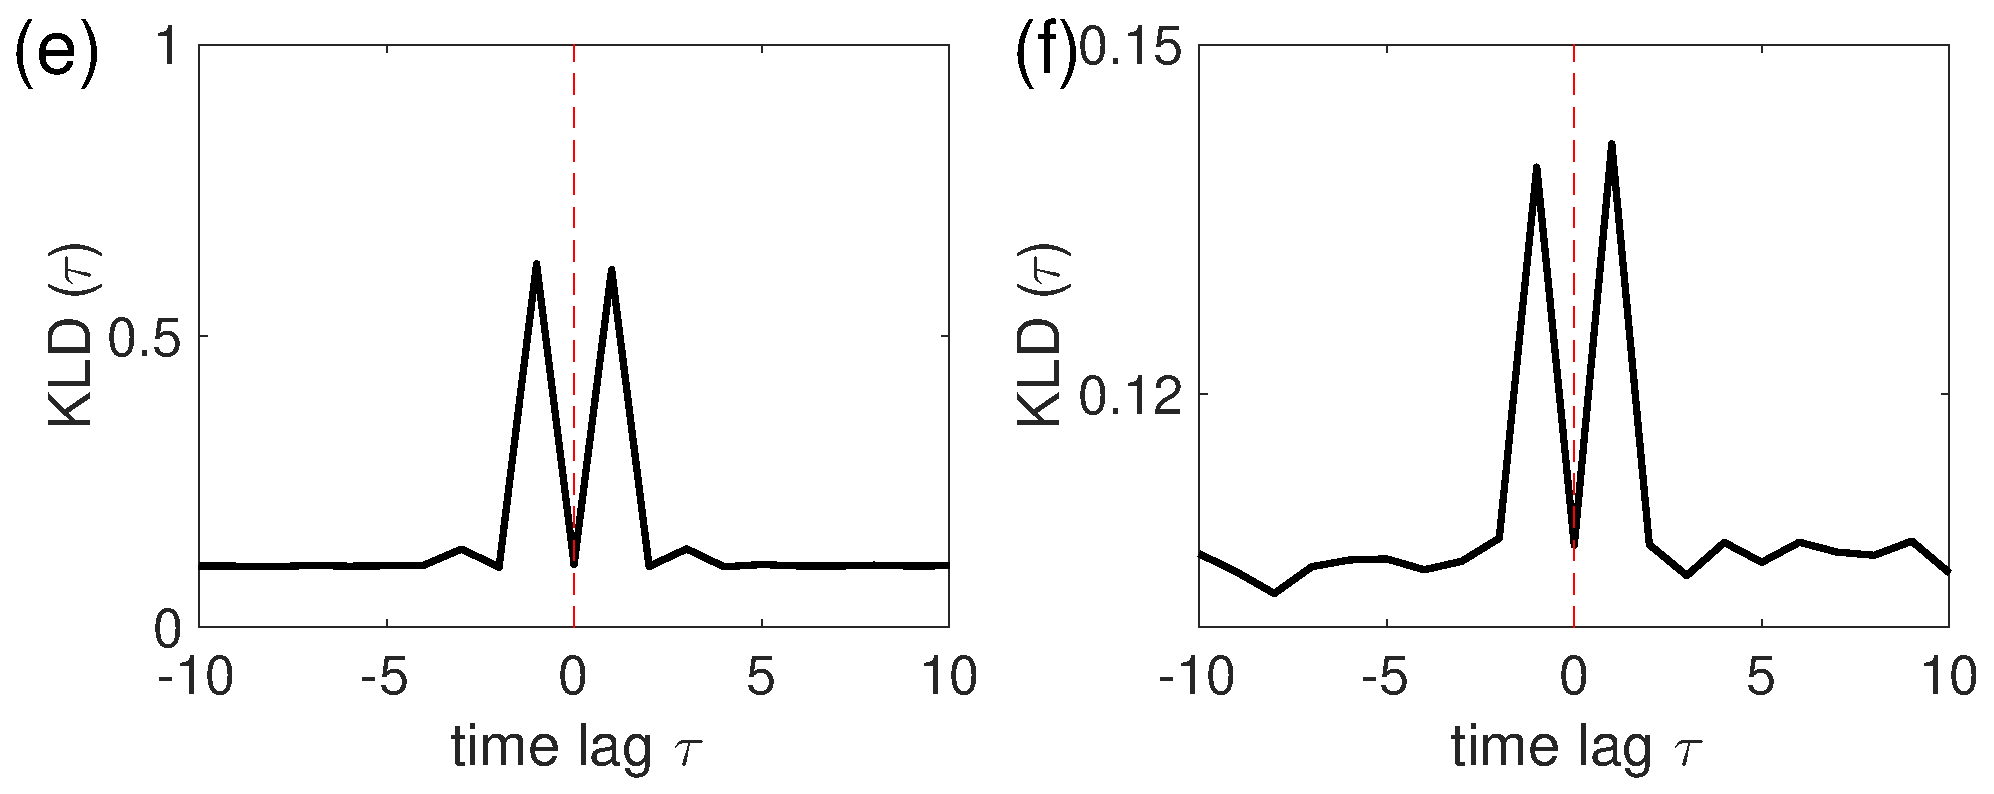
\includegraphics[width=\columnwidth]{KL_D.eps}
\caption{(Color online) Same as in Fig.~\ref{fig:stdHeqB} but for Eq.~\eqref{eq:D}.   \label{fig:stdHeqD}}
\end{figure}

As a final example of coupled stochastic processes, we consider a more challenging case of asymmetric bidirectional interactions between $X$ and $Y$. More specifically, $X$ influences $Y$ at a delay $\tau = 2$ while the interaction from $Y$ to $X$ appears at a delay $\tau = 1$. The corresponding linear stochastic model reads as follows: 
\begin{equation} \label{eq:E}
D: \left \{ \begin{aligned}
x_{t+1} &= 0.3 y_{t} + \varepsilon_t, \\
y_{t+1} &= 0.5 x_{t-1} + \eta_t, 
\end{aligned}
\right.
\end{equation}
where $\{ \epsilon_t \}$ and $\{ \eta_t \}$ are again realizations of i.i.d. Gaussian noise. The nonlinearly transformed $\tilde{X}$ is defined as $\tilde{x}_{t} = \tanh{10 x_t}$. As in the previous three examples, in both the linear and nonlinear cases, the curves of $\sigma_{X \to Y}(\tau)$, $H_{X\to Y}(\tau)$ and $\text{KLD}(\tau)$ correctly identify two delays at $\tau = -1$ and $\tau = 2$ as shown in Fig.~\ref{fig:stdHeqE}. This correctly suggests that $X (\tilde{X})$ affects $Y$ at a delay of $\tau = 2$ while $Y$ influences $X (\tilde{X})$ at $\tau = 1$. 

\begin{figure}
	\centering
	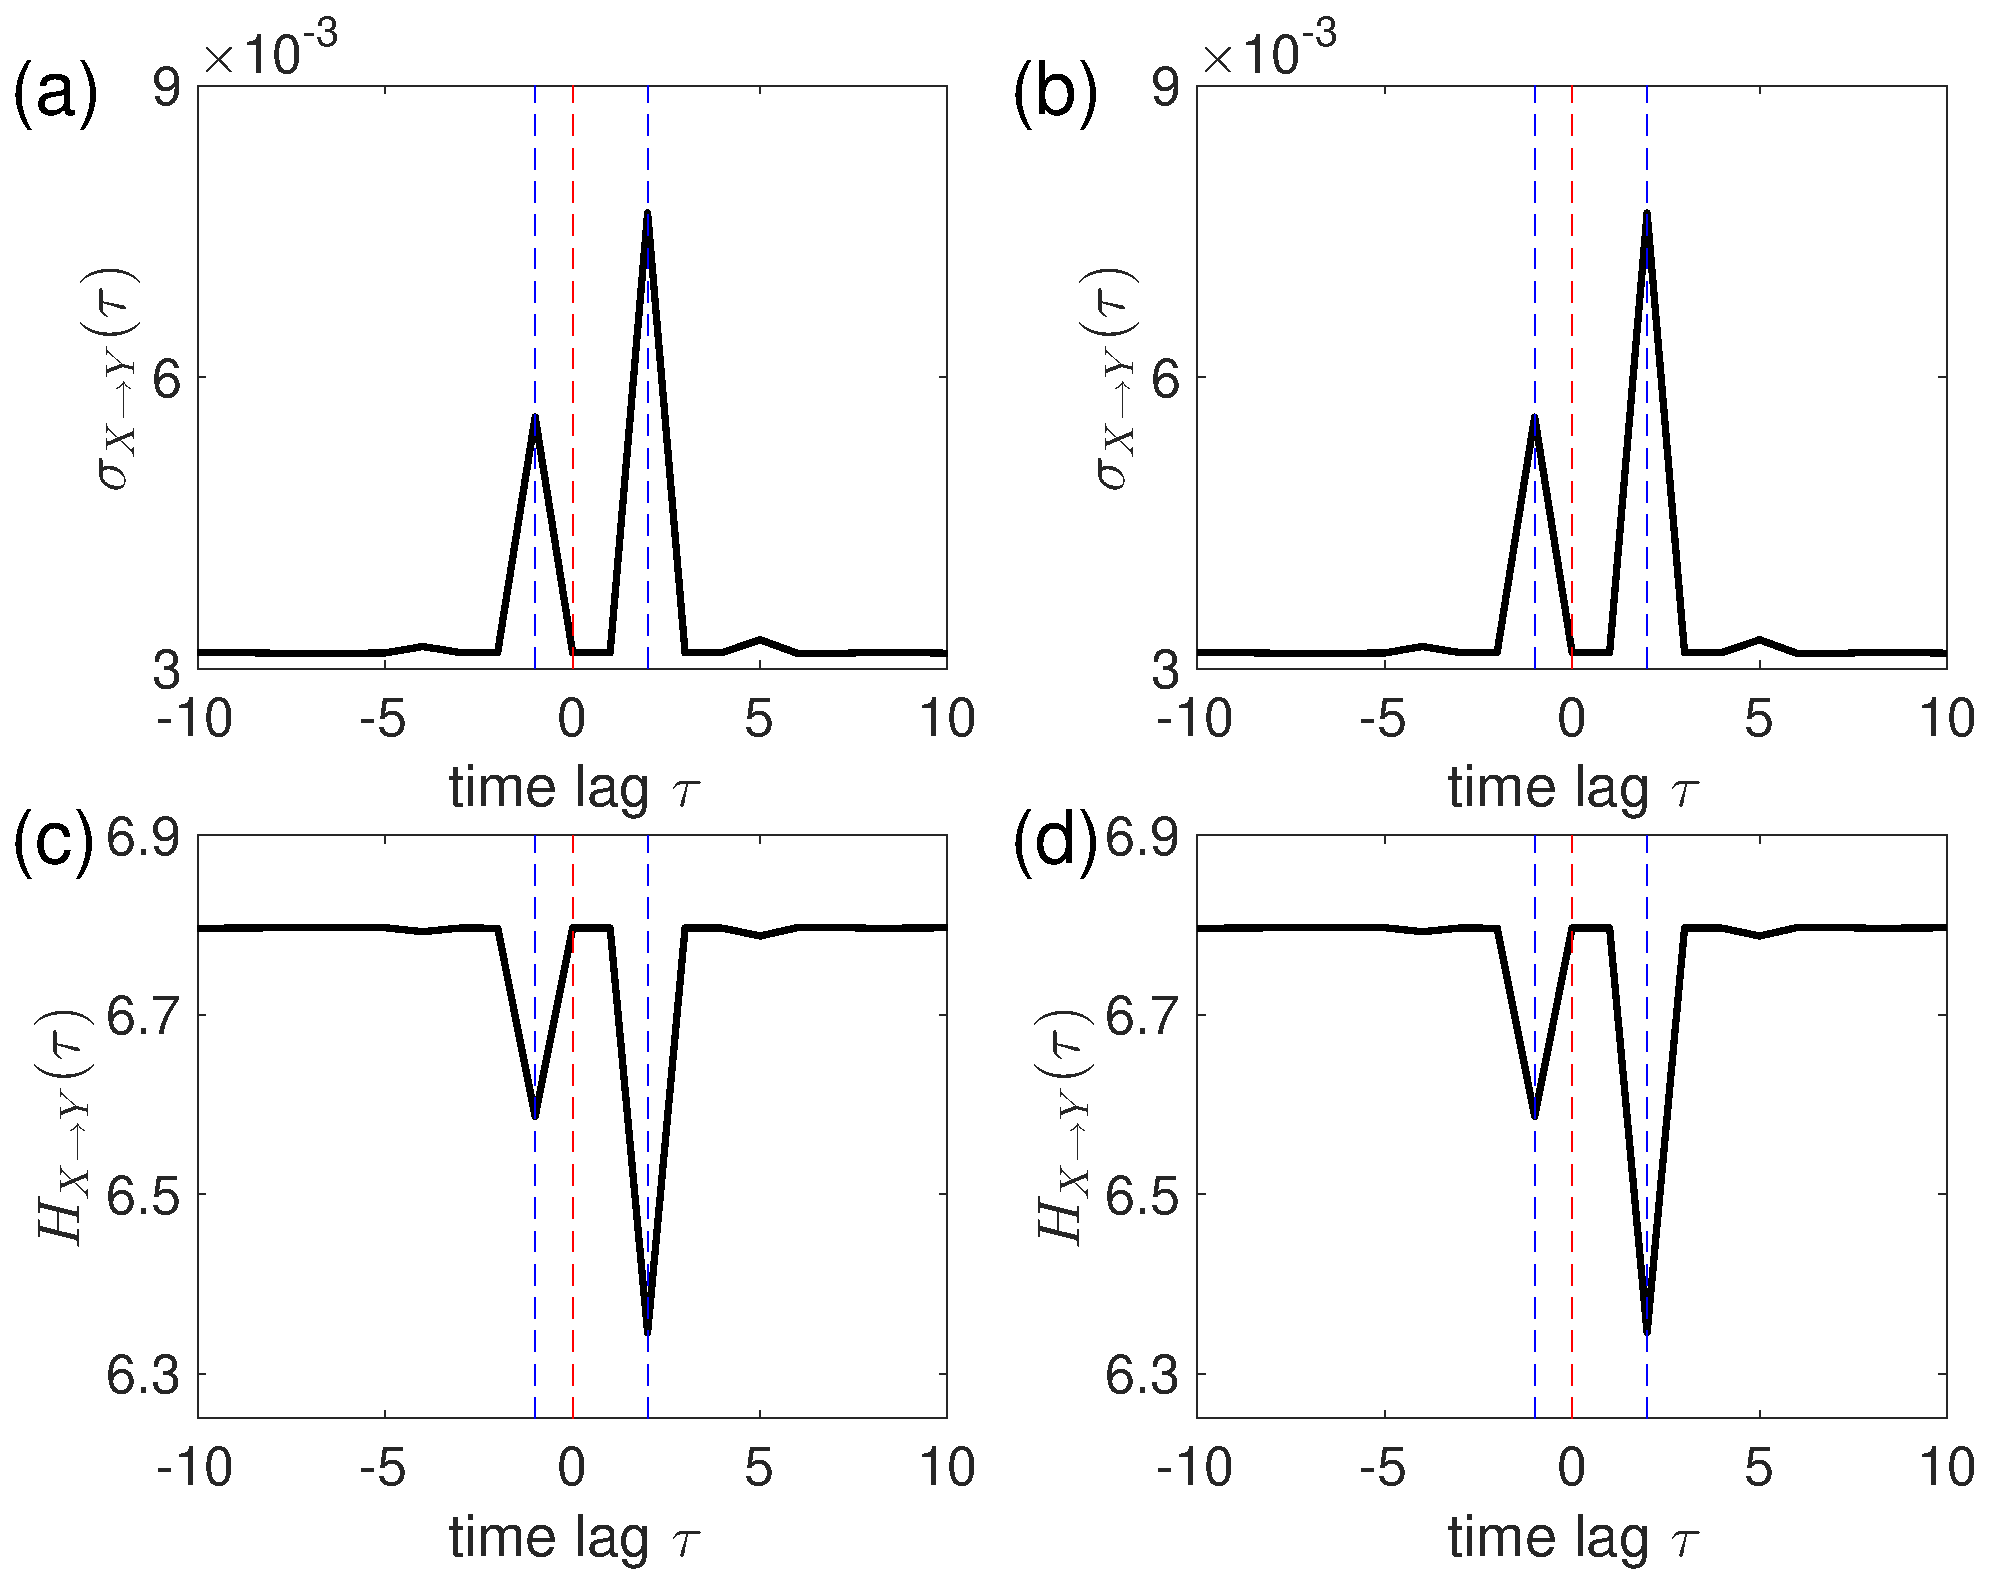
\includegraphics[width=\columnwidth]{E_E.eps}
	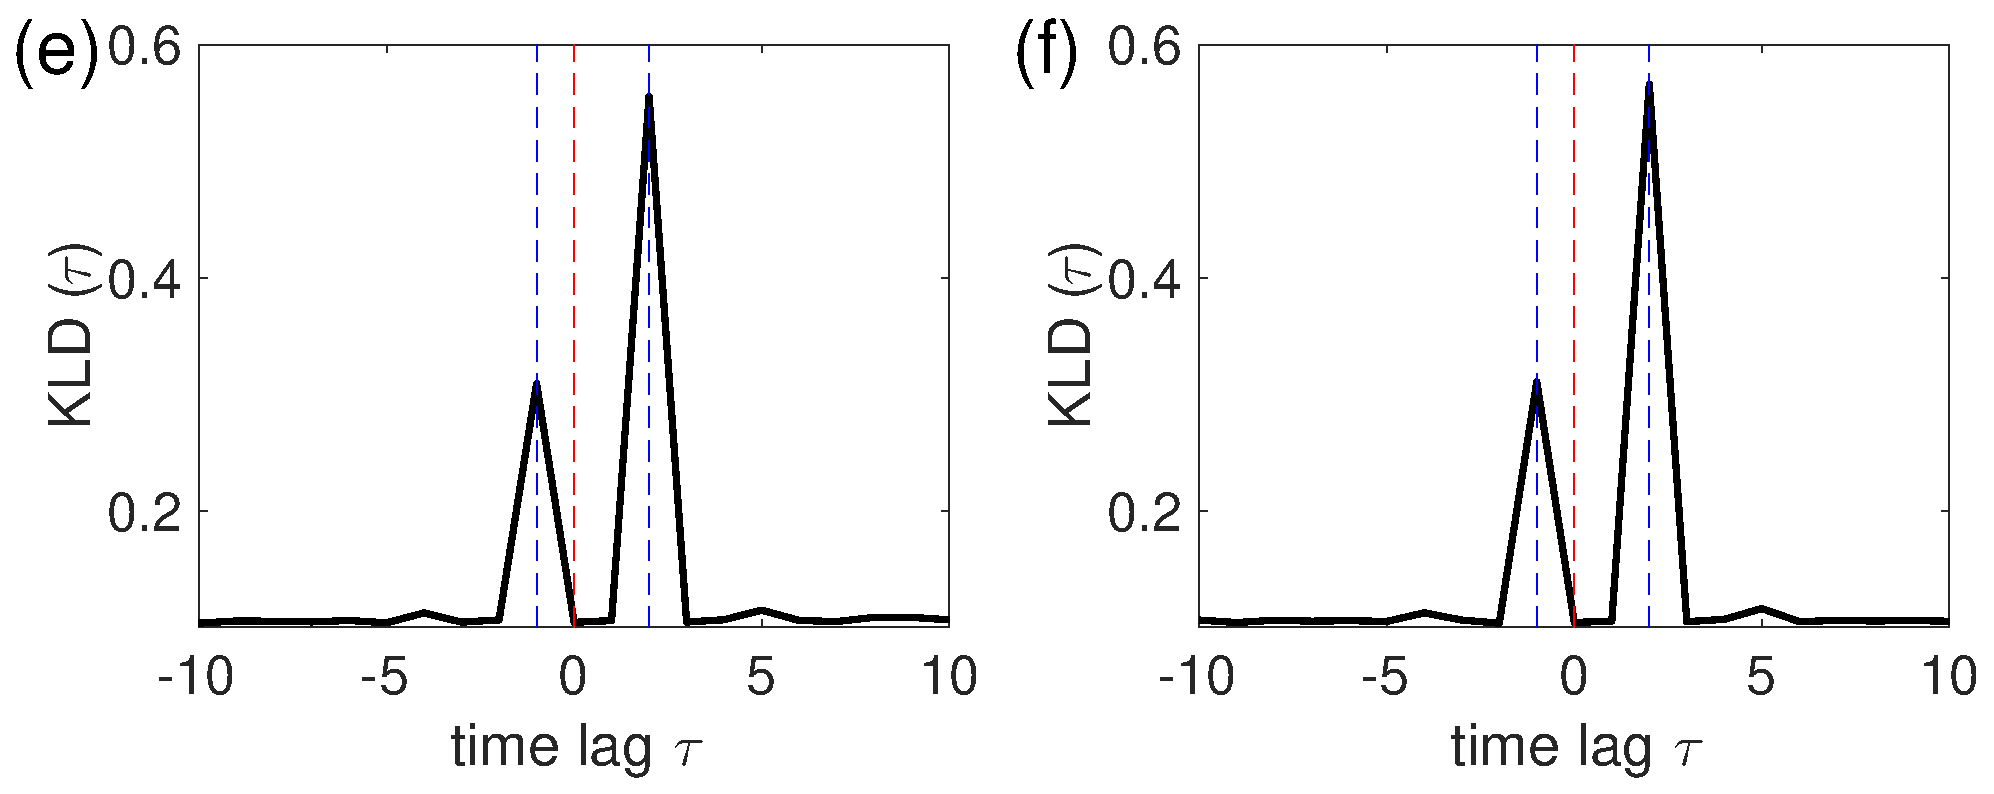
\includegraphics[width=\columnwidth]{KL_E.eps}
\caption{(Color online) Same as in Fig.~\ref{fig:stdHeqD} but for Eq.~\eqref{eq:E}. The two employed delays of $\tau = -1$ and $\tau = 2$ are additionally highlighted by vertical blue dashed lines. \label{fig:stdHeqE}}
\end{figure}

\subsection{Coupled nonlinear chaotic maps} \label{sec:henon}

As an additional numerical example, we further illustrate the performance of the proposed ordinal pattern co-occurrence complexity measures for detecting the coupling direction between two unidirectionally coupled nonlinear chaotic H\'enon maps~\cite{RomanoPRE2007}. In this case, the driving system $X$ reads 
\begin{equation} \label{eq:HX}
X: \left \{ \begin{aligned}
x_{t + 1}^{(1)} &= 1.4 - x^{(1)}_t x^{(1)}_t + b_1 x^{(2)}_t, \\
x_{t + 1}^{(2)} &= x_{t}^{(1)},
\end{aligned}
\right.
\end{equation}
while the response system $Y$ is given as 
\begin{equation} \label{eq:HY}
Y: \left \{ \begin{aligned}
y^{(1)}_{t + 1} &= 1.4 - [\mu x^{(1)}_t y^{(1)}_t+ (1 - \mu) y^{(1)}_t y^{(1)}_t] + b_2 y^{(2)}_t, \\
y^{(2)}_{t + 1} &= y^{(1)}_t,
\end{aligned}
\right.
\end{equation}
with $\mu$ being the coupling strength. In what follows, we consider cases of both, identical ($b_1 = b_2 = 0.3$) and nonidentical systems ($b_1 = 0.1, b_2 = 0.3$). Following ref.~\cite{RomanoPRE2007}, we restrict our discussion to values of the coupling strength within the interval $\mu \in [0, 0.6]$, since the coupling direction cannot be identified in the presence of identical synchronization which sets in at approximately $\mu = 0.65$. Mimicking the common situation in case of real-world observational time series, we assume that we have only observed the two scalar time series $\{ x^{(1)}_t \}_{t=1}^{N}$ (system $X$) and $\{ y^{(1)}_t  \}_{t=1}^{N}$ (system $Y$) instead of the full system. The resulting series are transformed into corresponding ordinal patterns using the embedding dimension $D = 5$ and time delay $\tau_d = 100$, i.e., the same parameters as for the stochastic processes in the examples discussed in Sec.~\ref{sec:GCs}. Again, we note that the results described in the following do not change qualitatively when other reasonable choices of embedding parameters are used (not shown). 

We choose four representative coupling strengths ($\mu = 0.2, 0.3, 0.4$ and $0.5$) and show the corresponding results in Fig.~\ref{fig:stdHeqXY}. The maximum values of $\sigma_{X \to Y}$ and $\text{KLD}(\tau)$ and the minimum values of $H_{X \to Y}$ become more pronounced when the coupling strength $\mu$ increases. Our numerical results demonstrate a monotonic increase in the amplitudes of the maxima of $\sigma_{X \to Y}$ and $\text{KLD}(\tau)$ along with a monotonic decrease in the minima of $H_{X\to Y}$ when increasing the coupling strength $\mu$, which are indicated by the left (black) vertical axes of Fig.~\ref{fig:stdHeqXY}(b,d,f). Furthermore, we observe that the positions of local maxima of $\sigma_{X \to Y}$ and $\text{KLD}(\tau)$ as well as the local minima of $H_{X\to Y}$ get gradually closer to zero, which originates from the synchronization process among the two coupled systems. Notably, the positions of these maxima/minima are shifted towards zero time lag when $X$ and $Y$ are identically synchronized. We define an index $X \to Y$ to capture the coupling direction by the positions of global maxima $\tau_{max}$ of $\sigma_{X \to Y}(\tau)$ and $\text{KLD}(\tau)$ (global minima $\tau_{min}$ of $H_{X \to Y}(\tau)$), where a positive value of this index reflects a coupling direction from $X$ to $Y$. When increasing the coupling strength $\mu$ as shown by the right (blue) vertical axes in Fig.~\ref{fig:stdHeqXY}(b,d,f), we conclude that the unidirectional coupling direction from $X$ to $Y$ has been well captured by the positive values of this coupling direction index. We note that the fluctuations of this index at rather weak interactions ($\mu \in [0, 0.02]$) are due to the imprecise identification of the maxima of $\sigma_{X\to Y}(\tau)$ and $\text{KLD}(\tau)$ (minima of $H_{X\to Y}(\tau)$). In turn, the index $X \to Y$ drops to zero values when $\mu \gtrsim 0.52$ because the coupling strength gets close to the complete synchronization regime \cite{RomanoPRE2007}. 

\begin{figure}
	\centering
	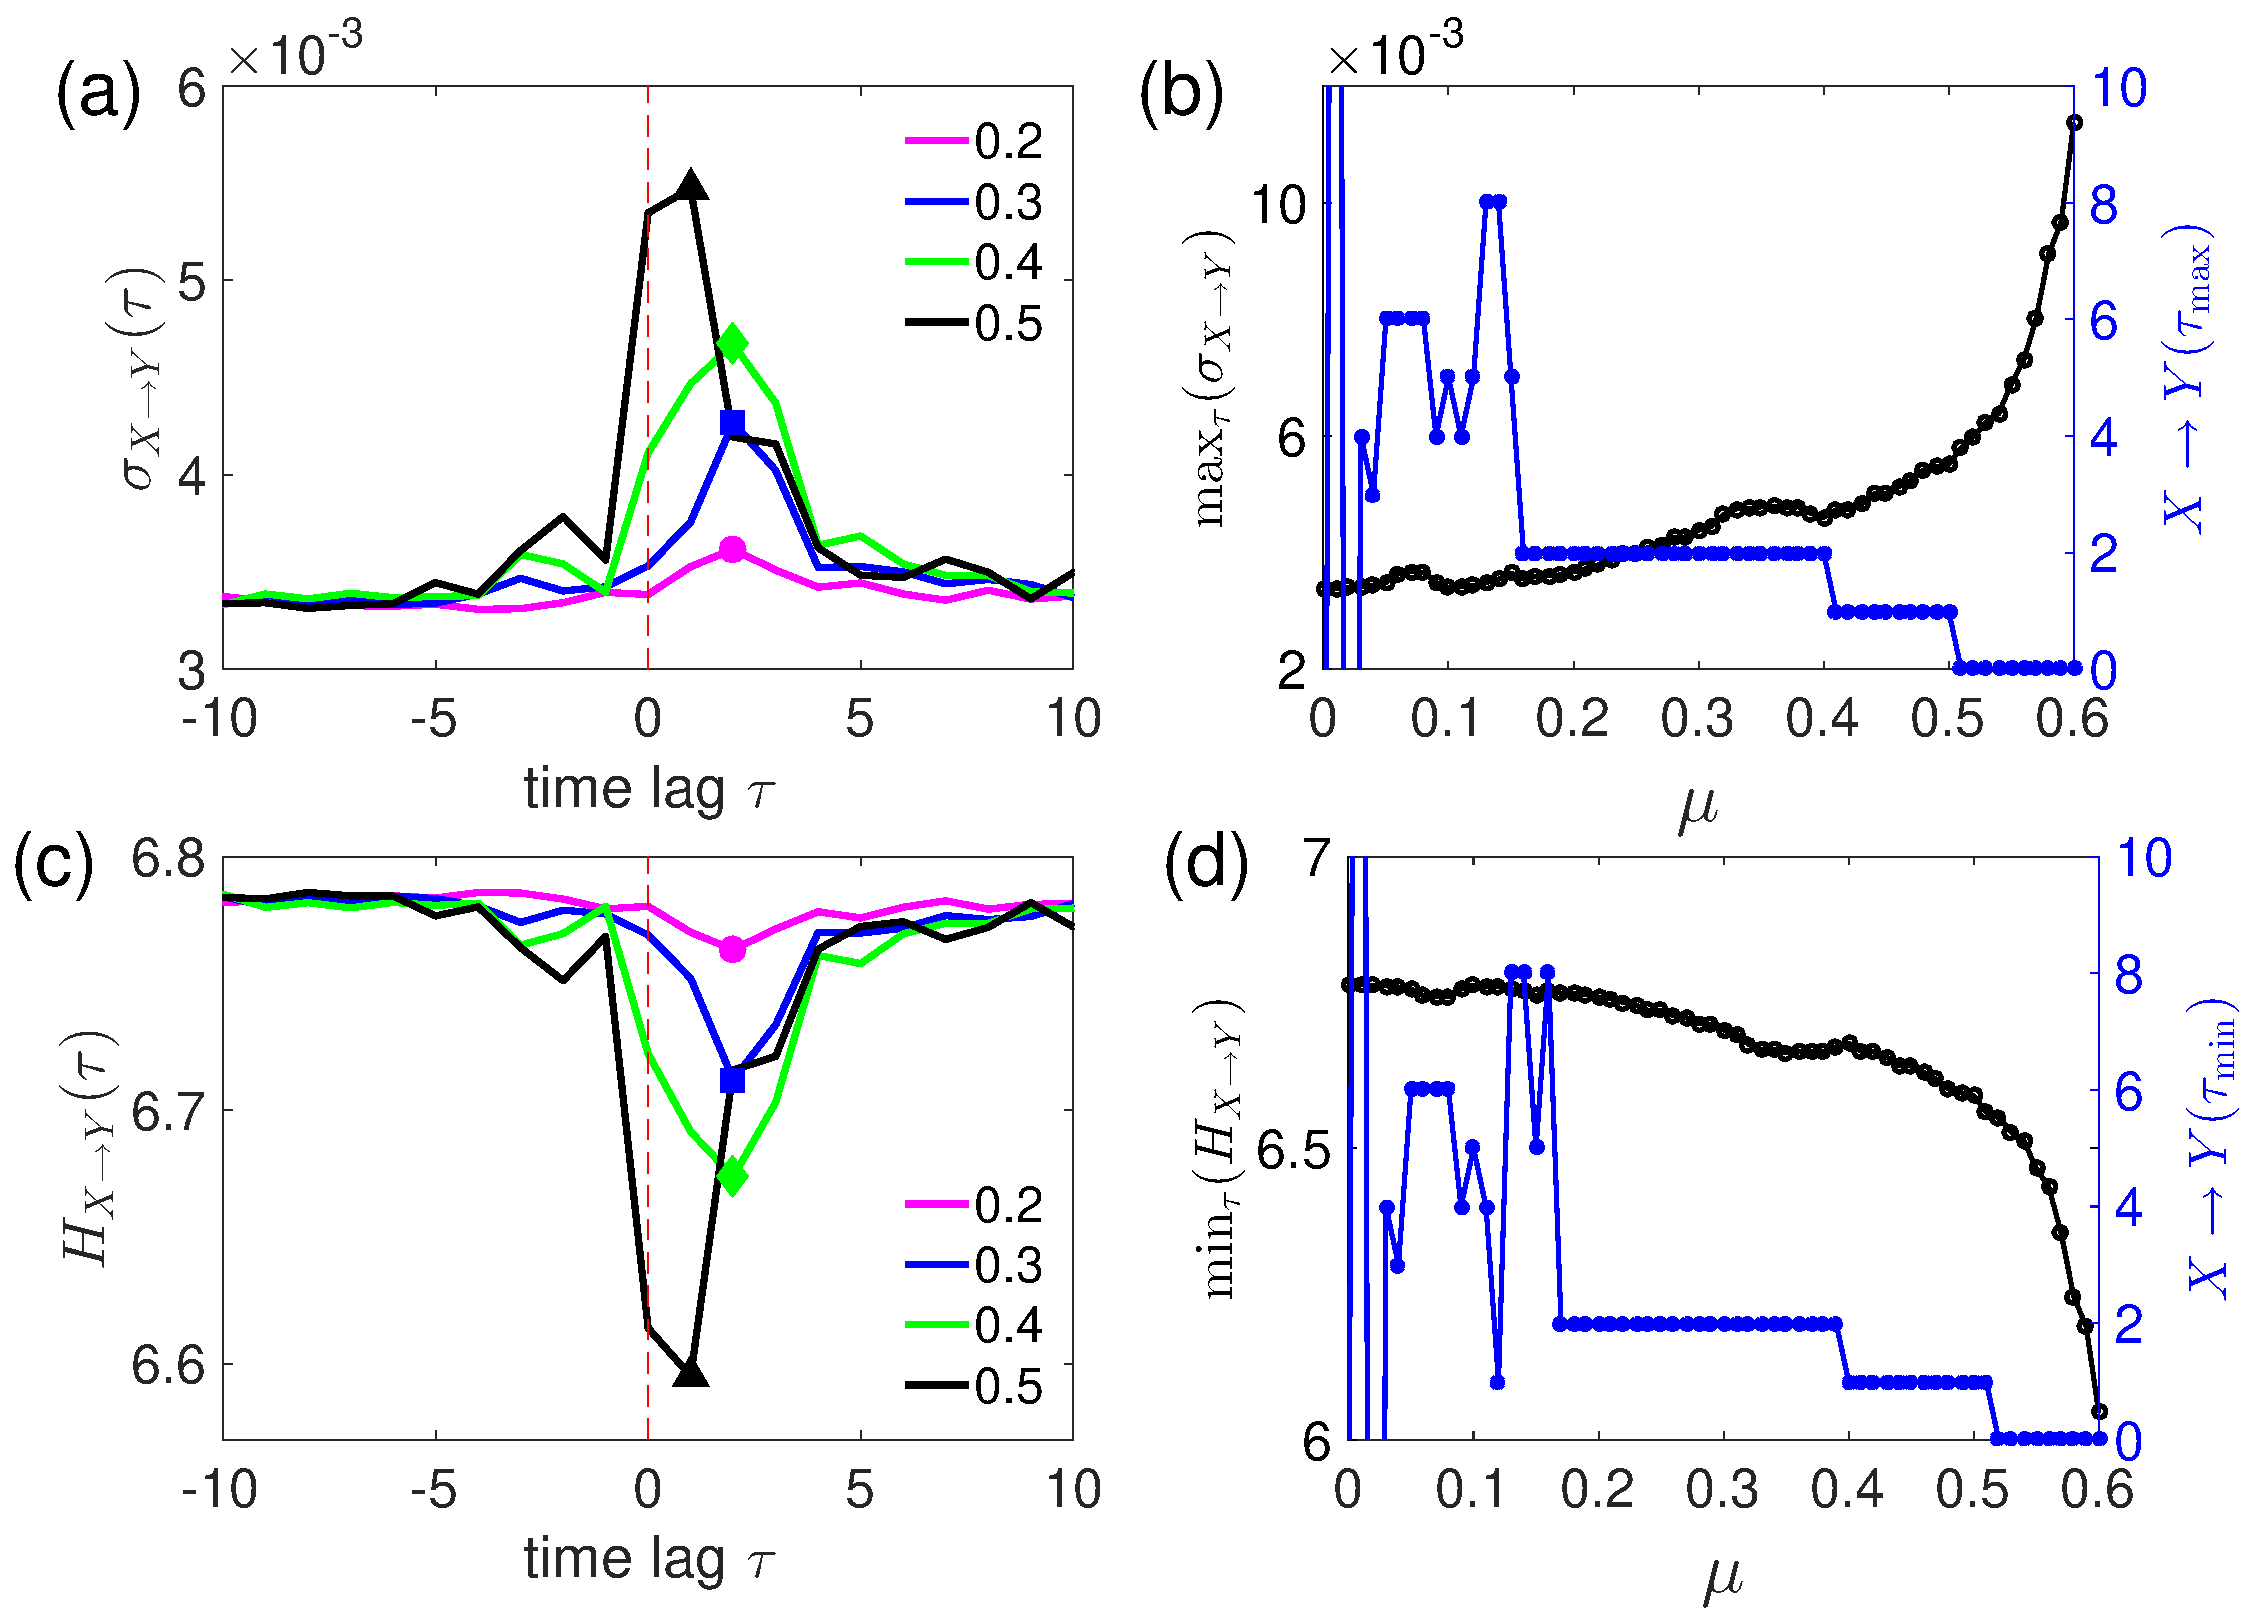
\includegraphics[width=\columnwidth]{henonMaps.eps}
	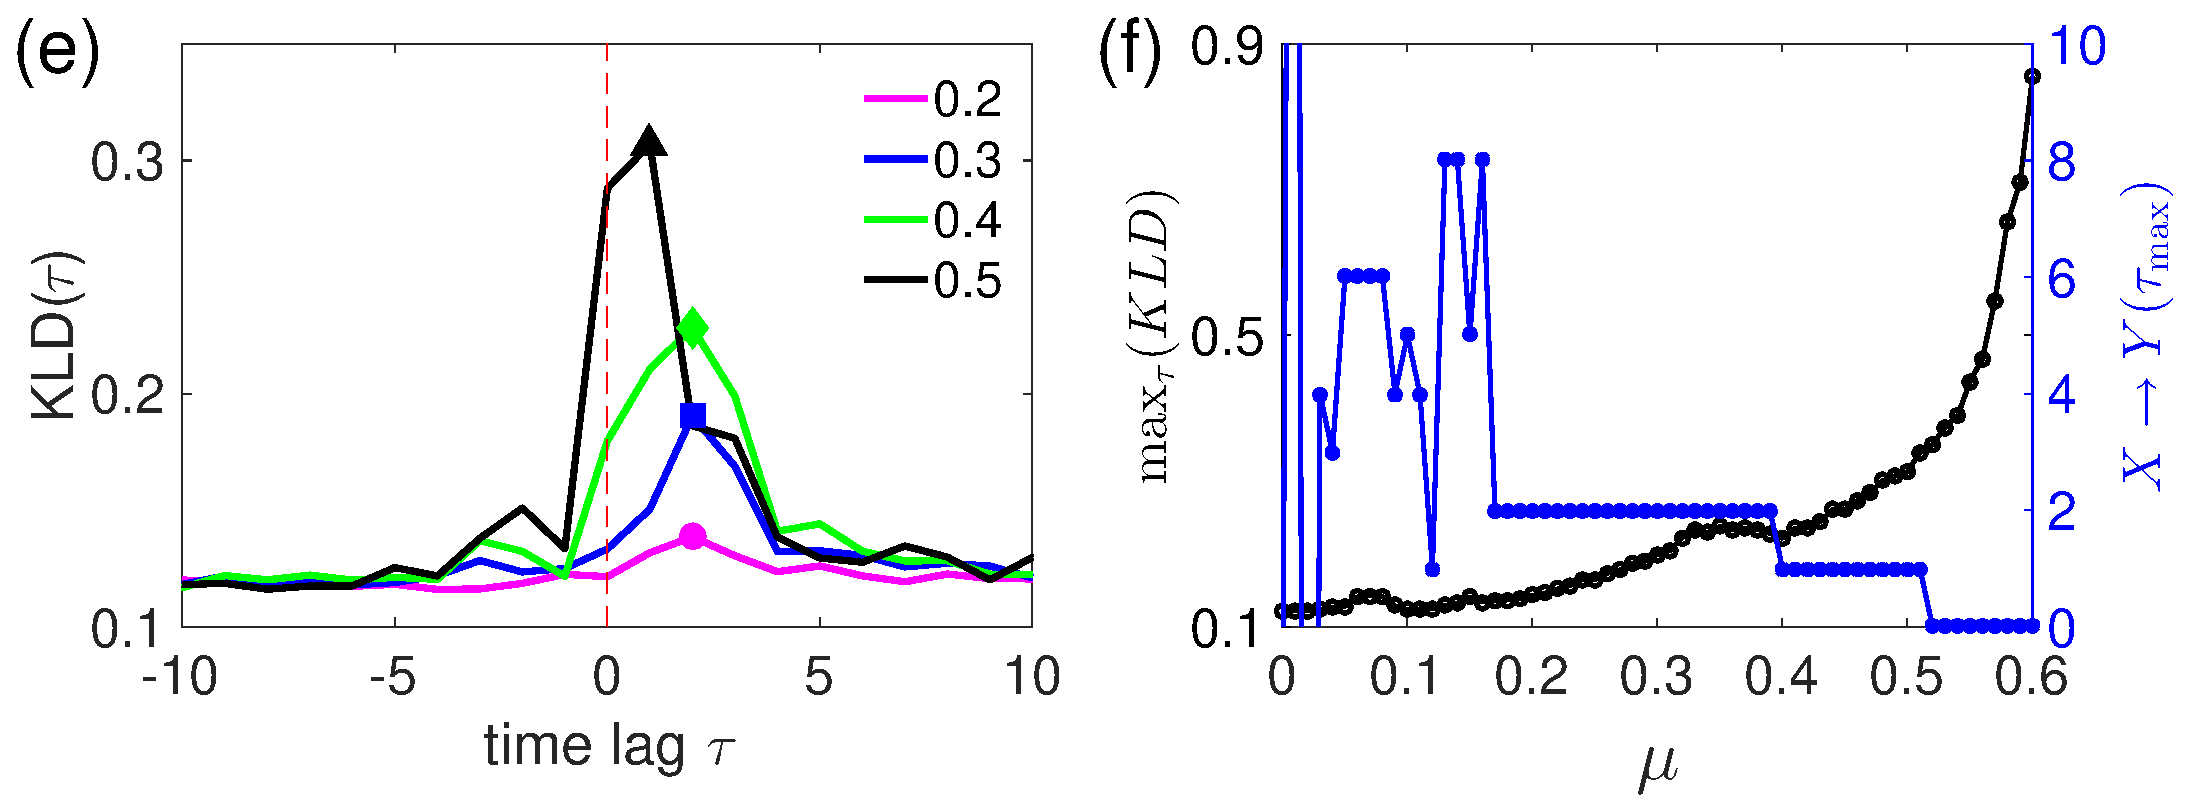
\includegraphics[width=\columnwidth]{henon_KL.eps}
\caption{(Color online) (a,c,e) Same as in Fig.~\ref{fig:stdHeqB} but for the case of unidirectionally coupled H\'enon maps (Eqs.~\eqref{eq:HX} and \eqref{eq:HY}). We show four cases of coupling strengths $\mu = 0.2, 0.3, 0.4$ and $0.5$ as indicated by the legends. The corresponding maximum/minimum values of the three measures $\sigma_{X \to Y}$ (a), $H_{X \to Y}$ (c), and $\text{KLD}$ (e) are annotated by different types of symbols. (b,d,f) The left vertical axes indicate the maximum/minimum values of the corresponding ordinal pattern co-occurrence complexity measures while the right one provides the values of the coupling direction index $X \to Y$ (i.e., the positions of the respective maxima/minima of the three considered measures). \label{fig:stdHeqXY}}
\end{figure}


\subsection{Sample size dependence of complexity measures}
{\color{red}So far, all three complexity measures extract the coupling directions correctly. As discussed above, $\sigma_{X\to Y}(\tau)$ is expected to be zero, while $H_{X\to Y}(\tau)$ converges to a maximal value $H_{X \to Y} = \log_2 D!$ if all $D!$ patterns are distributed uniformly in both $X$ and $Y$, which is the case for two uncoupled systems. These empirical expectations may be subjected to the marginal distributions of patterns. In contrast, we do expect zero values of $\text{KLD}(\tau)$ for uncoupled systems even }if the marginal frequency distributions of the corresponding ordinal patterns are not exactly the same, the KLD measure (Eqs.~\ref{eq:localKLD},\ref{eq:globalKLD}) is defined such that it should asymptotically approach zero in the case of uncoupled systems. 

In turn, we expect positive non-zero values of KLD for two coupled systems, in particular at the positions of the true interaction delays. However, due to the finite length of any given pair of time series, one may observe small non-zero KLD values in the case of non-causal delays, as has been shown in our numerical results discussed above (cf.\ Figs.~\ref{fig:stdHeqB}-\ref{fig:stdHeqE}). 

{\color{red}In order to further study such finite sample size effects on the obtained complexity measures, we reconsider the coupled stochastic processes from Sec.~\ref{sec:GCs} and choose two specific time lags $\tau$, one corresponding to the position of the maximal values of $\sigma$ and KLD (minimal of $H$) indicating causal interaction, while the other is coinciding with the position of some non-causal delay with small $\sigma$ and KLD value (maximal of $H$). In the following, we report the numerical results for the KLD measures only since this discriminator is more statistically motivated. Anyway, we note that the same asymptotical results have been obtained for the other two measures of $\sigma_{X\to Y}$ and $H_{X\to Y}$, as shown in Figs. S1 -- S4 in the Supplementary Materials (SM). }

For all four previously studied systems, we observe different asymptotic behaviors of KLD at these two different delays. Notably, when increasing the time series length $N$, the KLD values at the causal delays show convergence to non-zero values, while dropping to zero approximately as $1/N$ at the non-causal delays. This feature is clearly visible for all four stochastic processes with both, unidirectional and bidirectional coupling as shown in Fig. \ref{fig:sampleSizeBCDE}. {\color{red}In all cases, the results are reliable if time series length is larger than $N \gtrsim 10000$. }  

\begin{figure}
	\centering
	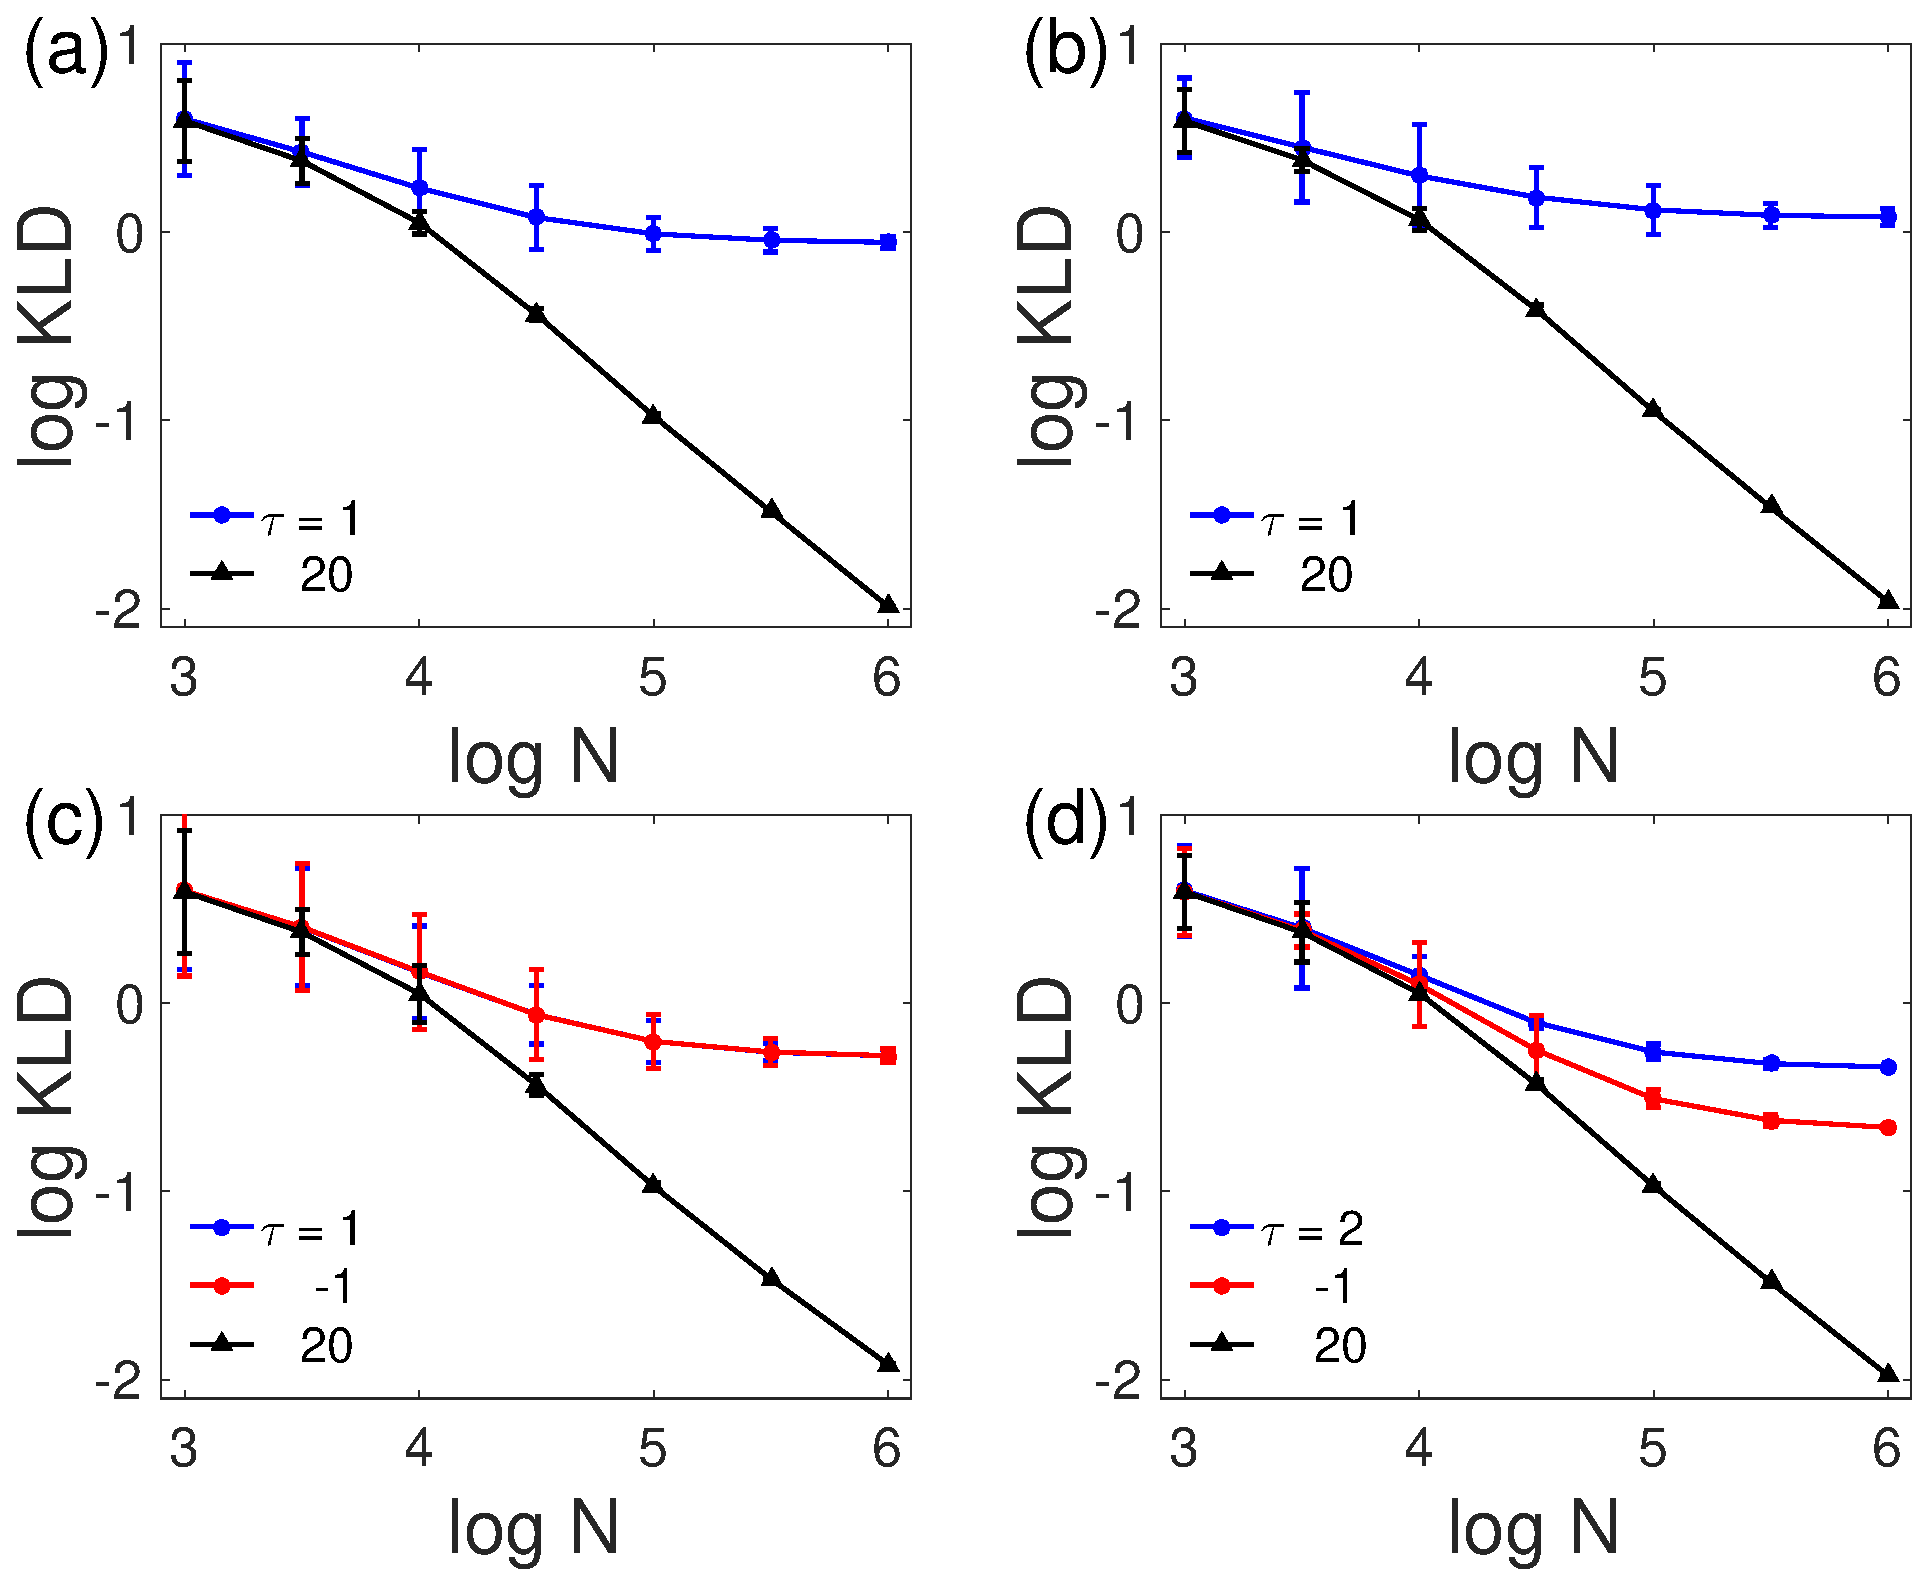
\includegraphics[width=\columnwidth]{kld_lengthBCDE.eps}
\caption{(Color online) Double logarithmic plot of the dependence of KLD on the sample size $N$ for the optimal (causal) lags (blue/red) and some non-causal lag (black) for the four cases of coupled linear-stochastic systems: (a) Eq.~\eqref{eq:B} (unidirectional), (b) Eq.~\eqref{eq:C} (unidirectional), (c) Eq.~\eqref{eq:D} (symmetric bidirectional), (d) Eq.~\eqref{eq:E} (asymmetric bidirectional). In (c,d), the values for both causal delays are shown. Errorbars correspond to the standard deviation (linear scale) over 20 independent realizations.  \label{fig:sampleSizeBCDE}}
\end{figure}

Qualitatively equivalent results have been obtained for the two coupled chaotic H\'enon maps from Sec.~\ref{sec:henon} as shown in Fig.~\ref{fig:sampleSizeHenon}. Here, we have again studied four different values of the coupling strength, $\mu = 0.2$, $0.3$, $0.4$ and $0.5$, and chosen the coupling delays based on the results of Fig.~\ref{fig:stdHeqXY}, corresponding to the respective maximum KLD values on the one hand, and some non-causal delay with low value of KLD on the other hand. {\color{red}As for cases of coupled stochastic processes, the distinctive convergence results are reliable if length $N \gtrsim 10^4$. The special case is for} the rather weak coupling $\mu = 0.2$, the different convergence behavior of KLD is visible for $N \gtrsim 10^6$. Similar results are found for the three other coupling strengths as shown in Fig.~\ref{fig:sampleSizeHenon}(b-d). {\color{red}Similar results have been obtained for $\sigma_{X\to Y}$ and $H_{X\to Y}$, as shown in Figs. S3 and S4 in SM. }
\begin{figure}
	\centering
	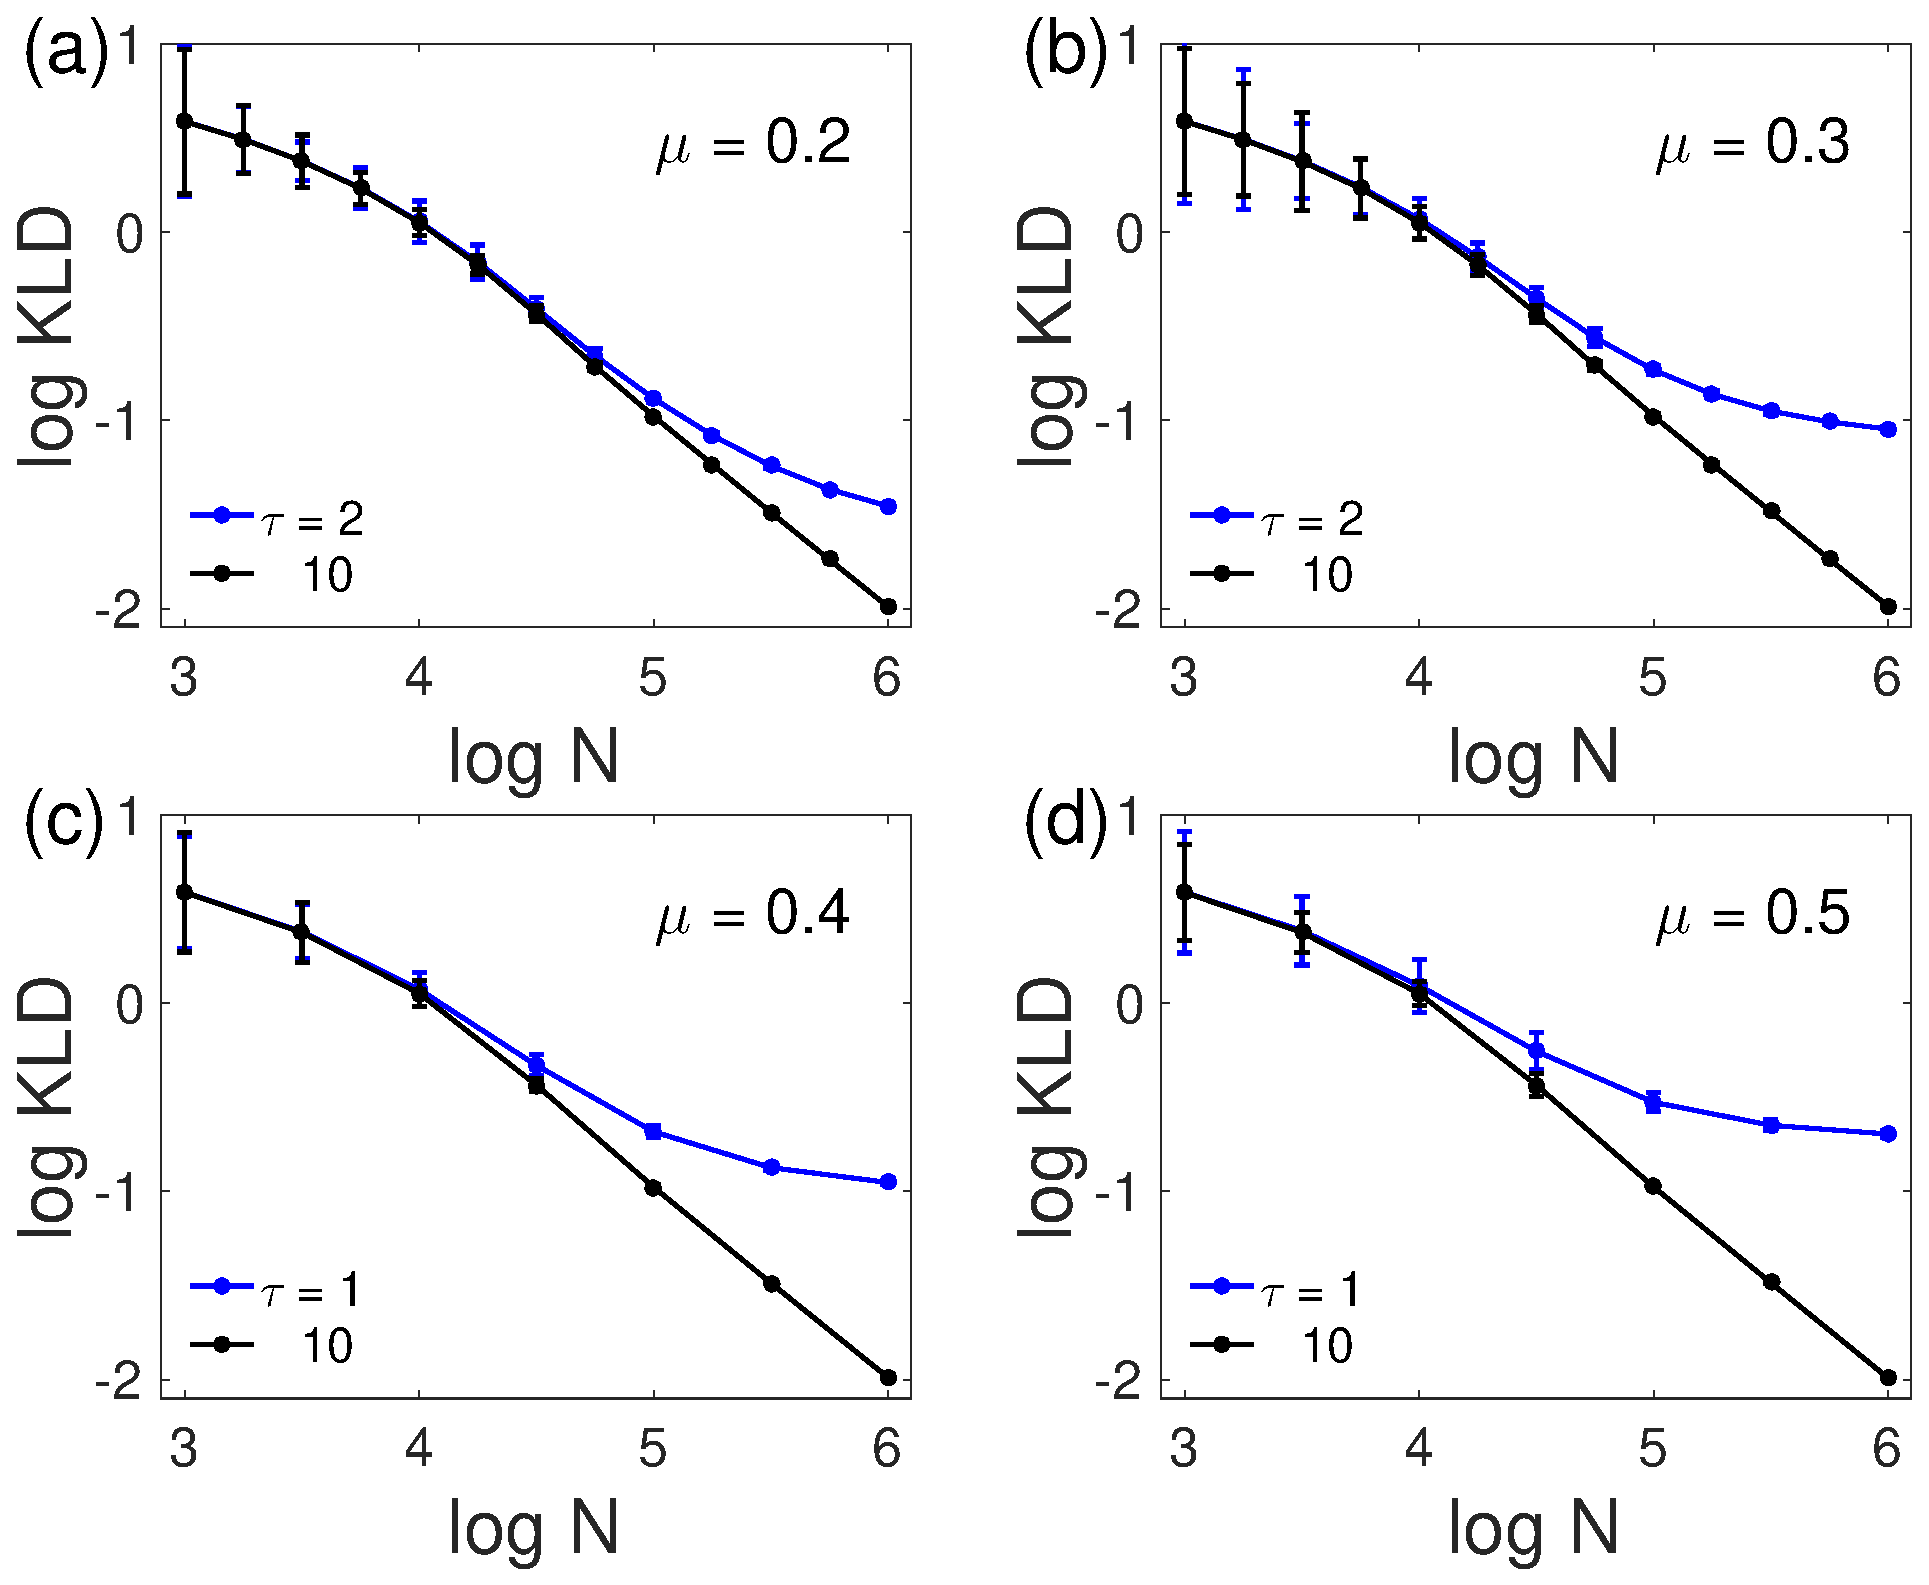
\includegraphics[width=\columnwidth]{kld_lengthHenon.eps}
\caption{(Color online) Same as in Fig. \ref{fig:sampleSizeBCDE} but for the two coupled H\'enon maps at four different coupling strengths $\mu$: (a) $\mu=0.2$ (b) $0.3$, (c) $0.4$, and (d) $0.5$. The blue lines show the behavior at the delay corresponding to maximum KLD, while the black ones show the values for a non-causal delay of $\tau=10$. \label{fig:sampleSizeHenon}}
\end{figure}

Taken together, we conclude that the small non-zero {\color{red}complexity} values at non-causal delays are indeed due to the finite length of the studied time series. This suggests a straightforward strategy for obtaining confidence bounds for the computed {\color{red}complexity} values by comparing them with those for surrogate data constructed by shuffling or bootstrapping the underlying time series individually. We leave a more detailed exploration of this idea as a subject of future work.


\section{Real-world example}  \label{sec:exp}
In this section, we apply the proposed methodology to characterize the statistical interdependence between temperature records from two distant meteorological stations. Specifically, we study two long-term daily temperature records from Oxford (Great Britain) and Vienna (Austria) as previously investigated in ref.~\cite{Rybski2003} by means of phase synchronization measures. The data used here are publicly available via the KNMI Climate Explorer (\url{http://climexp.knmi.nl}) and cover the period from 1 January 1901 to 31 December 2010. Missing values have been ignored in the subsequent analysis, and the mean annual cycles (estimated by the mean temperature values of each station for a given calendar day) have been subtracted from both records to avoid the otherwise dominating effect of this regular variability mode. 

In general, temperature records like those used here are characterized by some irregular alternation between colder and warmer phases due to large-scale atmospheric patterns (corresponding to high and low pressure centers, respectively), which in the case of western-to-central Europe travel in the majority of situations in eastward direction {\color{red}\cite{Barnston1987}}. According to the typical spatial extent of such pressure systems, it is likely that both considered sites experience similar variability patterns, yet with some mutual delay {\color{red} which is often termed as teleconnection}. Indeed, Rybski \emph{et~al.}~\cite{Rybski2003} reported phase synchronization between both stations with the record obtained in Oxford leading that from Vienna by on average 1 day. It should be noted, however, that one should not expect a simple strong linear correlation between both series, since the typical climatology at both sites is clearly different (i.e., more marine -- and, hence, variable -- versus more continental -- and, hence, persistent) and potentially affected by different circulation regimes.

Taking the two temperature series as described above, we construct the corresponding bipartite OPTN. Subsequently, we compute the transition complexity measures $\sigma_{X\to Y}$, $H_{X\to Y}$ and $\text{KLD}_{X\to Y}$ for different time lags, which are shown in Fig.~\ref{fig:stdHeqTemp}(a)-(c). When mutually shifting both series with respect to each other by several days in any of the two possible directions, we find a marked yet relatively slow decrease of $\sigma_{X\to Y} (\tau)$, $H_{X\to Y} (\tau)$ and $\text{KLD}_{X\to Y}$, which can most likely be explained by the known persistence of air temperature time series, together with the expectation that the actual delay should be time-dependent and, thus, distributed over several values. Altogether, the most significant values of all three measures are attained at a mutual delay of $\tau=1$ day, with the values at $\tau=2$ days being only slightly less prominent. In summary, our analysis identifies an interaction delay between the respective local temperature variations of 1 to 2 days (with Oxford leading Vienna), which is consistent with the previous results of phase synchronization analysis~\cite{Rybski2003}. This coupling delay is reasonable since temperature variations in Oxford arising from general atmospheric circulation patterns are typically propagated eastward and reach Vienna about 1 to 2 days later, which corresponds to the average propagation speed of frontal systems in the northern mid-latitudes west-wind zone {\color{red}\cite{Barnston1987}}. 

\begin{figure}
	\centering
	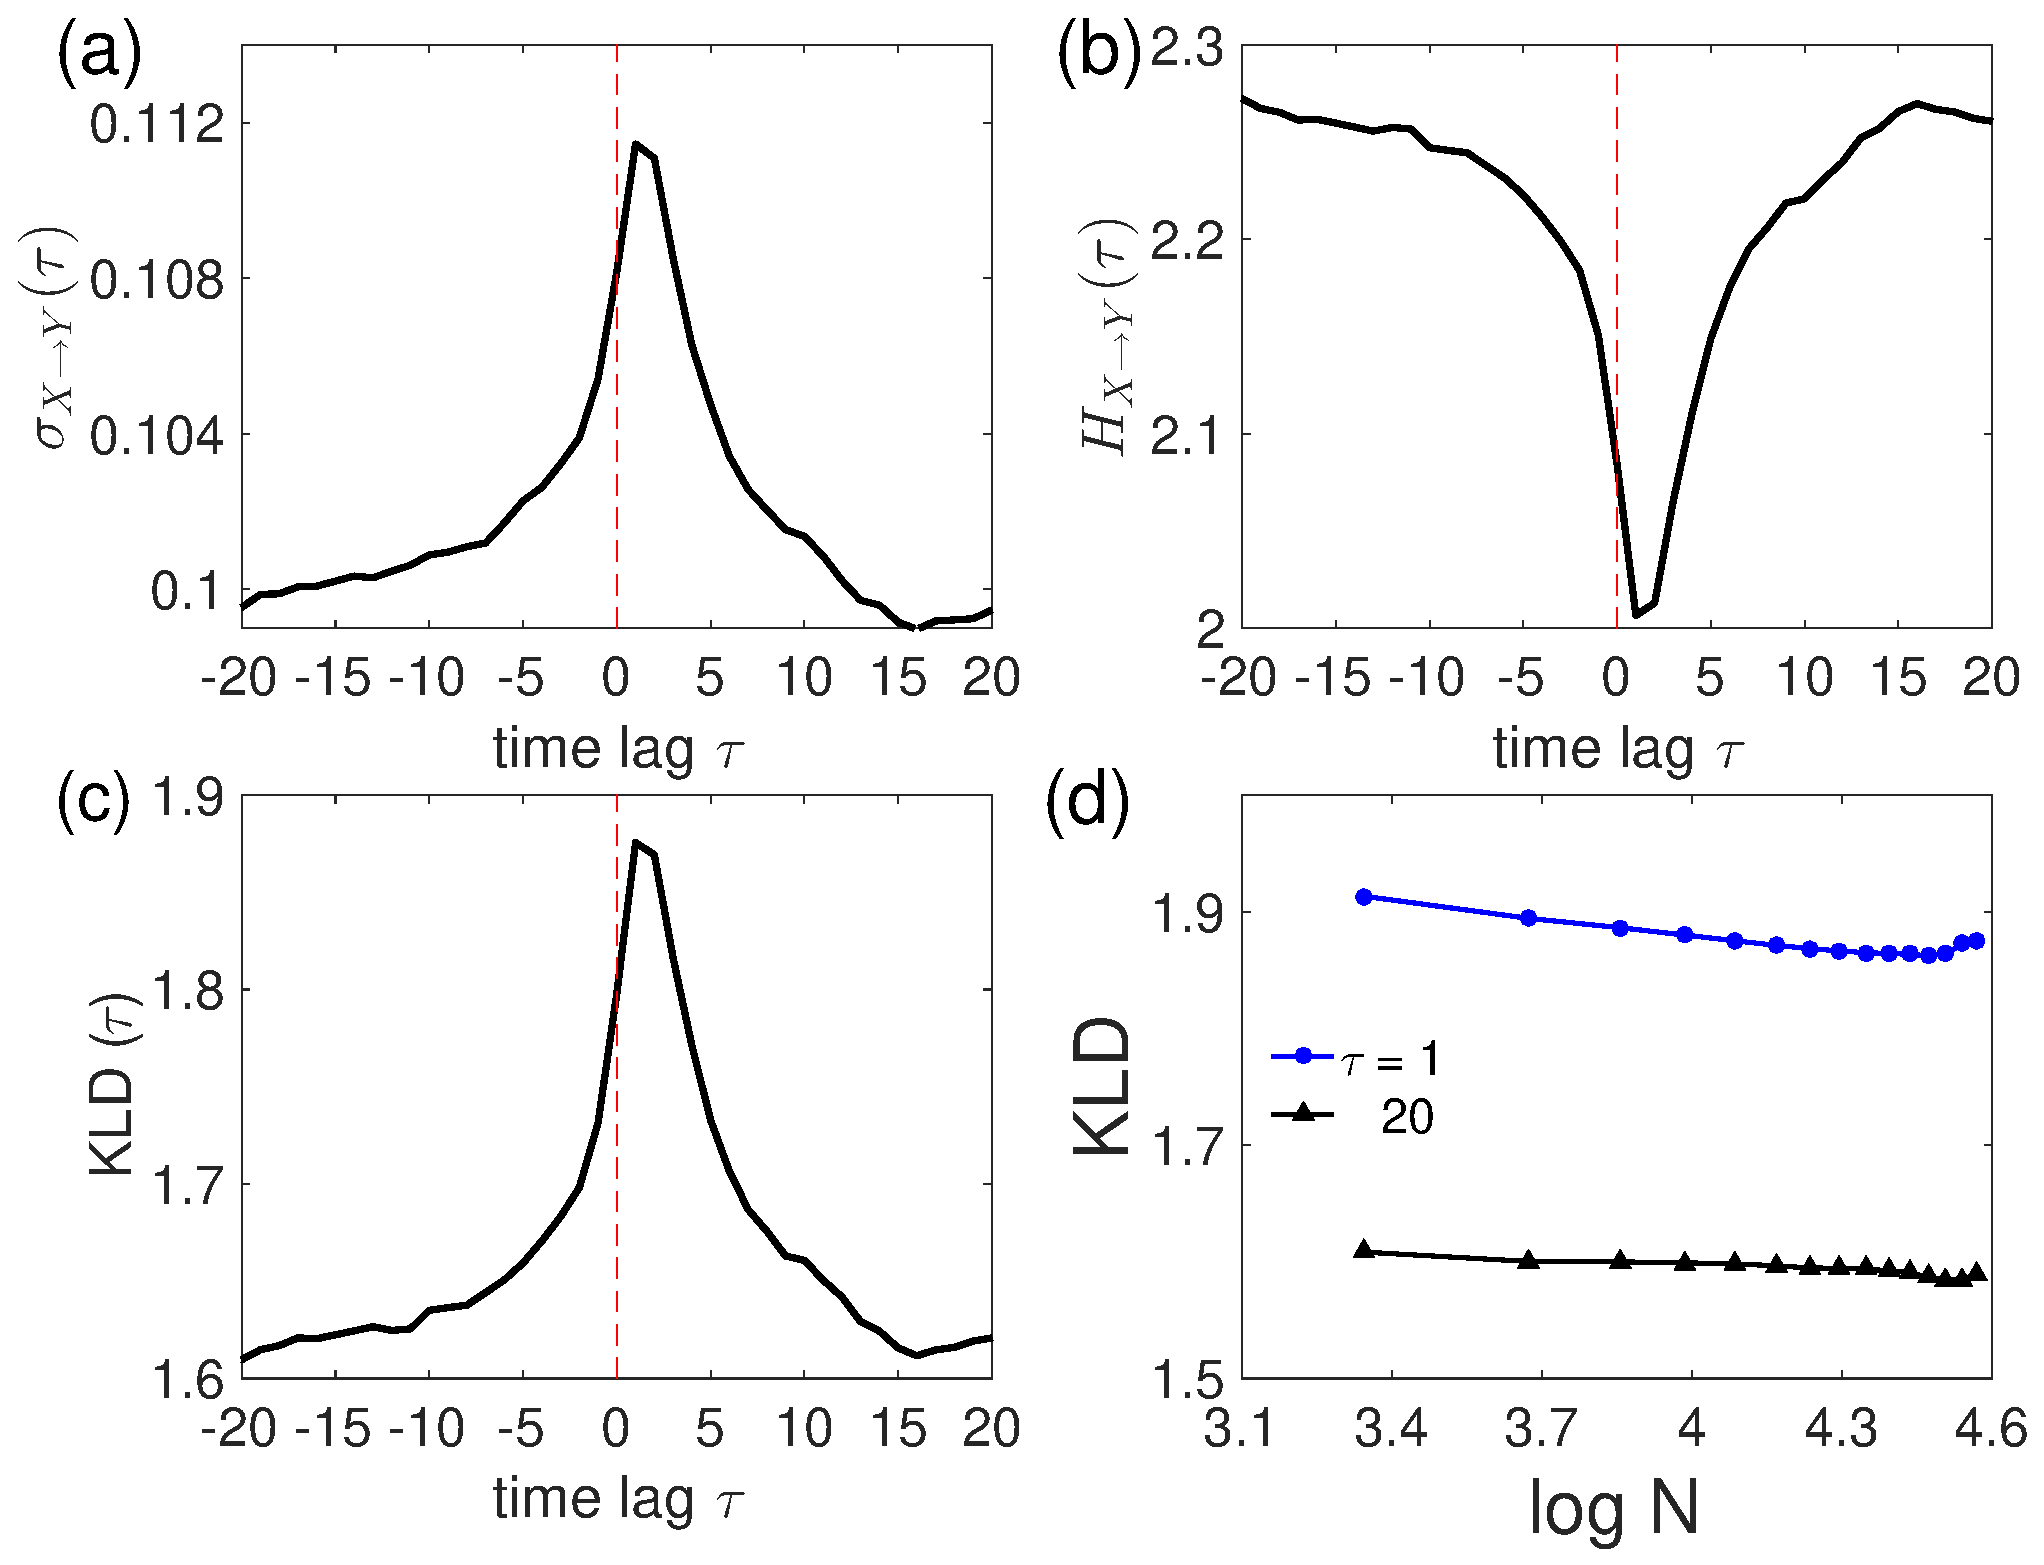
\includegraphics[width=\columnwidth]{E_temperature.eps}
\caption{(Color online) OPTN based statistical coupling indicators between the daily surface air temperature records from Oxford ($X$) and Vienna ($Y$): (a) mean squared deviations of the conditional co-occurrence frequencies of ordinal patterns $\sigma_{X\to Y} (\tau)$, (b) global ordinal pattern co-occurrence entropy $H_{X\to Y}(\tau)$, and (c) Kullback-Leibler divergence $\text{KLD}(\tau)$. Dashed red vertical lines indicate the values for possible instantaneous interactions. (d) Dependence of KLD on the sample length $N$ at the optimal delay ($\tau=1$ day, blue) and some arbitrarily chosen large delay ($\tau=20$ days, black). 
\label{fig:stdHeqTemp}}
\end{figure}

In addition to the identification of the expected interaction delay between both temperature records, we have again studied the effect of the time series length on the estimated OPTN based coupling indicators for the example of KLD. For this purpose, pairs of time series values have been selected at random to form subsamples of arbitrary sizes. This kind of cross-validation procedure demonstrates the saturation of the obtained estimates at sufficiently large sample sizes (Fig.~\ref{fig:stdHeqTemp}(d)). Most importantly, the KLD values at the optimal interaction delay of $\tau=1$ day are consistently larger than those at any other delay that would not be justified by the underlying meteorological processes. However, there is a non-zero statistical relationship between both records even at a delay of 20 days, which is manifested in the saturation of KLD for this delay with increasing time series length $N$ instead of a gradual decrease as previously observed in our numerical model examples. {\color{red}Similar results have been obtained for $\sigma_{X\to Y}$ and $H_{X\to Y}$, as shown in Fig. S5 in SM. }

\section{Conclusions} \label{sec:con}

In summary, we have proposed to infer coupling direction and strength among pairs of dynamical systems by computing complexity measures from the resulting bipartite ordinal {\color{red}partition} transition networks (OPTNs). More specifically, we have estimated three quantitative characteristics capturing different aspects of the heterogeneity of conditional frequencies of occurrences in one time series relative to the second one. The first two measures, $\sigma_{X\to Y}$ and $H_{X\to Y}$, both characterize the degree to which the ordinal pattern distribution in one series can be attributed to prior information from the ordinal patterns of the second one. By contrast, the Kullback-Leibler divergence (KLD) between the conditional probability distribution of ordinal patterns $p(\pi_{j}^{Y} | \pi_i^{X})$ and the corresponding marginals $p(\pi_j^{Y})$ directly characterizes the presence of interdependence between the two underlying systems $X$ and $Y$. 

In order to identify the direction and relevant delay of coupling, we have performed a time-lagged analysis using all three measures, where the ordinal pattern series have been shifted relative each other by a given time delay $\tau$ prior to evaluating the associated empirical co-occurrence frequencies. Numerical results for unidirectionally and bidirectionally coupled stochastic processes and H\'enon maps have demonstrated the existence of pronounced signatures at the respective interaction delays, capturing the prescribed coupling directions successfully. In the particular case of coupling analysis for two temperature records from Oxford and Vienna, the ordinal pattern co-occurrence complexity measures have consistently identified interactions at a delay of 1 to 2 days, which suggests that these measures can be useful for analyzing interactions among real-world (noisy) time series. Follow-up studies should take up this problem to address more systematically the effect of observational noise on coupling identification using OPTN based complexity measures as compared to other existing statistical approaches serving similar purposes. The present work has provided a first proof-of-concept that concepts from ordinal time series analysis, combined with ideas from complex network theory, can provide complementary tools for coupling analysis. However, we have not attempted to study the performance of these measures along with that of other existing techniques, which remains as a subject of future studies.

Further open challenges along these lines of research include, but are not limited to characterizing dynamic variations of the coupling direction, i.e., situations where coupling changes its strength and possibly even direction as time evolves. A sliding window technique may be an option for such studies, however, the construction of proper OPTNs could be affected by the window sizes (relative to the time scales at which the coupling changes), which requires reliable estimation of the considered OPTN complexity measures. In addition, the generalization of the proposed measures to the case of more than two interacting processes is interesting, since complex interaction schemes are frequently observed across a vast range of scientific disciplines. Along with such examples, for instance, distinguishing direct from indirect coupling among three of more mutually coupled systems is still a subject of active research, which could be extended to further applications of OPTNs. 

\section*{Acknowledgement}
Parts of this work have been financially supported by the National Natural Science Foundation of China (Grant No. 11872182, 11875132, and 11835003) and the Natural Science Foundation of Shanghai (Grant No. 17ZR1444800 and 18ZR1411800). RVD acknowledges funding by the IRTG 1740/TRP 2011/50151-0 (funded by the DFG and FAPESP) and by the German Federal Ministry for Education and Research (BMBF) via the BMBF Young Investigators Group $\text{CoSy-CC}^2$: Complex Systems Approaches to Understanding Causes and Consequences of Past, Present and Future Climate Change (grant no. 01LN1306A).

%\bibliographystyle{unsrt}
\bibliography{PhysRep2018N,ref_Zhang}%,ref_reik}

\end{document}
